\documentclass[11pt]{article}
\usepackage[margin=1in]{geometry}
\usepackage{amsmath,amssymb}
\usepackage{graphicx}
\usepackage{booktabs}
\usepackage{hyperref}
\usepackage{xcolor}
\usepackage{natbib}
\usepackage{authblk}
\usepackage{multirow}
\usepackage{caption}
\usepackage{subcaption}

\definecolor{confirmed}{HTML}{059669}
\definecolor{refuted}{HTML}{E11D48}
\definecolor{partial}{HTML}{D97706}

\title{A sparse autoencoder atlas of the Novae spatial foundation model,\\with matched-null controls for interpretability claims}

\author[1]{Ihor Kendiukhov}
\affil[1]{University of T\"ubingen, Germany}

\date{\today}

\begin{document}
\maketitle

% ===================== ABSTRACT =====================
\begin{abstract}
Foundation models for spatial transcriptomics learn rich internal
representations of tissue architecture, but what biological knowledge
these representations encode remains unclear. We apply sparse
autoencoders~(SAEs) to Novae, a GATv2 graph neural network trained on
12~million spatially resolved cells, and recover \textbf{49{,}152
features} across all 12 internal surfaces of the model. Aggregator-
level features are overwhelmingly non-aligned with the model's SwAV
prototypes (0.0\% at $|\cos|\geq 0.7$) and the top-50 SVD axes
($\geq 99.4\%$ per surface), indicating pervasive superposition.

To quantify how much of Novae's representational structure is
genuinely spatial, we introduce two complementary graph-ablation
tests: replacing the Delaunay graph with self-loops suppresses
activation in 67\% of features, while a stricter feature-permutation
control (graph intact, node features shuffled across cells; 3 slides,
225k cells) flags 40\%; the \textbf{doubly-controlled intersection
(26\% of active features)} is our estimate of genuinely context-
dependent concepts. Prototype-reassignment ablations are calibrated
against a matched-magnitude random-direction null: \textbf{17 of 50}
tested features exceed the null's upper 95\% CI (direction-specific
load-bearing), 7 are below the null's lower 95\% CI, and 26 are
statistically indistinguishable from random matched-magnitude
perturbations. Cross-technology coherence is reported alongside a
raw-expression baseline: the SAE-feature Spearman
$\rho_\text{SAE} = 0.56$ between Xenium and MERSCOPE is matched by
$\rho_\text{raw} = 0.57$ on mean log-expression profiles, so the
continuous cross-tech signal is inherited from the overlapping panel
biology rather than added by the SAE; only 0.95\% of features are
strictly technology-specific.

Causal circuit tracing on a brain slide (24k cells, 90 source
features across 3 source layers) yields 439 directed edges. After
gap-normalizing by the number of traced (source, target) layer pairs,
edges per pair rise with gap in the current sample but every gap
$\geq 4$ is supported by a single source layer, so we describe the
attenuation profile as \emph{undetermined} until all source layers
are traced. Combinatorial triplet ablation gives
$R_{ABC} \in [0.957, 0.966]$ (paired bootstrap 95\% CI) for one
tested feature pair, a near-additive regime (deviation from
independence: 0.042) with small component effect sizes
($d \approx 0.04$). Spatial-gradient steering on the colon crypt-
villus axis shows a \textbf{22 pp} change in villus-directional push
between attenuation and amplification ($\alpha = 0.5 \to 5.0$:
$39\% \to 61\%$), the appropriate effect-size statement given the
asymmetric unperturbed distribution. An interactive atlas at
\url{https://biodyn-ai.github.io/novae-atlas/} makes features
browsable by markers, cell types, niches, and circuits.
\end{abstract}

% ===================== INTRODUCTION =====================
\section{Introduction}

\subsection{The interpretability gap in spatial biology}

Spatial transcriptomics technologies---10x Xenium \citep{xenium},
MERFISH \citep{merfish}, and CosMx---have transformed tissue biology
\citep{marx2021,moses2022,rao2021}, routinely profiling hundreds
of genes at subcellular resolution across entire tissue sections.
Foundation models trained on these data, such as Novae
\citep{novae}, learn to represent each cell in the context of its
spatial neighborhood: a graph neural network \citep{kipf2017,velickovic2018,li2022gnn}
aggregates gene-expression signals across Delaunay-triangulated
neighbors, and a SwAV \citep{swav} contrastive head clusters the resulting embeddings into
512 hierarchical ``niche prototypes.'' The model performs well on
downstream tasks (cell-type prediction, spatial domain segmentation),
but \emph{what it has learned internally} is opaque. The 512
prototypes offer a coarse view; the 10-layer GATv2 \citep{gatv2}
encoder may represent far richer structure---cell-cell interactions,
microenvironment gradients, technology-invariant tissue patterns---but
this structure is inaccessible through the prototype head alone.

\subsection{Sparse autoencoders as a microscope for neural networks}

Sparse autoencoders (SAEs) have recently emerged as a tool for
\emph{mechanistic interpretability}: the discipline of reverse-engineering
the computations inside trained neural networks
\citep{olah2020,elhage2021,elhage2022superposition,cunningham2023,bricken2023}. An SAE is
an overcomplete dictionary that decomposes a model's hidden activations
into a sparse set of independently meaningful \emph{features}---directions
in activation space that each correspond to a human-interpretable concept.
Because neural networks pack many more concepts into their hidden
dimensions than the dimension count would na\"ively allow (a phenomenon
called \emph{superposition}), linear methods like PCA fail to find these
features; the SAE's sparsity constraint forces each feature to isolate a
single concept.

The approach was originally developed for large language models
\citep{sharkey2022,bricken2023,conmy2023,bills2023,templeton2024,marks2025,gao2024}.
\citet{sae_atlas} adapted it to single-cell foundation models
(Geneformer \citep{geneformer}, scGPT \citep{scgpt}; see also
\citealt{yang2022,hao2024,rosen2023}), demonstrating that SAE features in these models
correspond to specific cell types, pathways, and regulatory programs.
We extend this line of work to the \emph{spatial} domain, where graph
neural networks create a fundamentally different inductive bias:
representations are shaped not just by a cell's own genes, but by its
neighbors' identities and spatial arrangement.

\subsection{This work}

We train TopK SAEs \citep{gao2024} on every internal layer of
\texttt{novae-human-0} (the human checkpoint of Novae) and apply a
comprehensive validation suite that tests 10 preregistered hypotheses
about the model's representations. The key question is: \emph{does
Novae's spatial graph architecture produce representations that are
qualitatively different from cell-identity-only models?} Our graph-ablation
experiment (H8), spatial-coherence analysis (H7), and cross-technology
coherence are uniquely enabled by the spatial setting and
could not be performed on non-spatial models like Geneformer.
Beyond hypothesis testing, we perform causal circuit tracing---zeroing
individual features and measuring their downstream effects across GATv2
layers---to discover directed causal relationships between spatial
concepts. This extends the circuit-tracing methodology of
\citet{sae_atlas} from transformer residual streams to graph attention
networks, where causal effects propagate through the spatial tissue
graph.

% ===================== METHODS =====================
\section{Methods}

\subsection{Model and data}

Novae \citep{novae} is a 32M-parameter GATv2 graph neural network
with 10 attention layers, trained via SwAV contrastive learning on
$>$12 million cells from human and mouse spatial-transcriptomics
datasets. We use the \texttt{novae-human-0} checkpoint, which
embeds each cell as a 64-dimensional vector (the ``aggregator''
output) that integrates the cell's own gene expression with its
spatial neighbors' signals through iterative graph attention.

Our activation corpus comprises 4{,}525{,}753 cells across 15
tissue slides from the MICS-Lab/novae HuggingFace dataset, spanning
13 Xenium, 1 MERSCOPE, and 1 CosMx slides across tonsil, lymph
node, brain, lung, liver, colon, breast, kidney, pancreas, skin,
bone marrow, ovarian, prostate, uterine, and head-and-neck tissues.

\subsection{Activation extraction and SAE training}

We hook 12 internal surfaces: the CellEmbedder output ($d=512$),
10 GATv2 convolutional layers ($d=128$ for layers~0--8, $d=64$ for
layer~9), and the aggregator ($d=64$). Each SAE consists of a linear
encoder that maps a $d$-dimensional hidden state into an overcomplete
$n$-dimensional feature space, a TopK sparsification step that retains
only the $k$ highest-magnitude features per input (setting the rest to
zero), and a linear decoder that reconstructs the original hidden state
from the sparse code \citep{gao2024,makhzani2014}. SAEs are trained at
$32\times$ expansion with MSE reconstruction loss
(Table~\ref{tab:sae_specs}), producing 49{,}152 features in total
across all surfaces.

\begin{table}[ht]
\centering
\caption{SAE specifications per surface. All SAEs achieve $\geq$80\%
variance explained; the aggregator achieves 99.8\%.}
\label{tab:sae_specs}
\begin{tabular}{lcccc}
\toprule
Surface & $d_\text{in}$ & $n_\text{features}$ & $k$ & Var.\ expl. \\
\midrule
Cell embedder & 512 & 8{,}192 & 32 & 91.4\% \\
Conv 0--8 & 128 & 4{,}096 & 32 & 81--94\% \\
Conv 9 & 64 & 2{,}048 & 16 & 90.3\% \\
Aggregator & 64 & 2{,}048 & 16 & 99.8\% \\
\bottomrule
\end{tabular}
\end{table}

\subsection{Feature characterization}

Each SAE feature is characterized through five lenses:
\begin{enumerate}
\item \textbf{Top genes}: the 20 genes with highest mean expression
      in the feature's top-0.1\% cells (by activation magnitude),
      ranked by fold-change over the corpus baseline.
\item \textbf{Enrichment analysis}: Enrichr \citep{enrichr}
      against GO Biological Process \citep{go2021}, KEGG \citep{kegg2000},
      Reactome \citep{reactome2020}, PanglaoDB \citep{panglao}, and
      CellMarker \citep{cellmarker2019}.
\item \textbf{Niche assignment}: Fisher enrichment against Novae's
      hierarchical domain labels at three resolutions (7, 12, 20
      Leiden \citep{leiden} clusters).
\item \textbf{Module discovery}: Leiden community detection on the
      pointwise-mutual-information co-activation graph of features.
\item \textbf{Superposition geometry}: cosine similarity to the
      top-50 SVD axes of each surface's activation matrix.
\end{enumerate}

\subsection{Causal validation suite}
\label{sec:methods_validation}

We apply the following causal and confound-control tests, organized
into primary tests (1--6), matched-magnitude and architectural nulls
(7--9), and baseline comparisons (10--11).

\paragraph{1. Self-loop graph ablation.}
We replace each cell's Delaunay spatial graph with self-loops
(\texttt{scipy.sparse.eye}), re-run Novae's forward pass, and
SAE-encode the result. For each feature, \emph{contextual dependency}
$= (\bar{|a|}_\text{full} - \bar{|a|}_\text{iso}) / \bar{|a|}_\text{full}$
measures how much the feature's activation drops when neighborhood
information is removed. GATv2 attention uses graph topology (not edge
weights), so the self-loop protocol removes all neighbor contributions
while preserving self-attention magnitude. Three regimes (bare,
degree-normalized, degree-preserving rewire) are tested and give
identical results.

\paragraph{2. Feature-permutation graph ablation.}
A stricter ablation that separates loss of aggregation from loss of
neighbor content: we keep the Delaunay graph intact but permute node
features (\texttt{adata.X}) across cells. Each cell then receives
attention-weighted messages from its real spatial neighbors, but the
content of those messages is random. Feature-permutation dependency
is computed identically to (1). This control requires a fresh forward
pass per slide and is run on 3 slides (brain, kidney, pancreas;
225{,}867 cells).

\paragraph{3. Prototype-domain ablation.}
For the 50 highest-confidence features, we zero each feature in the
SAE code, decode the ablated representation, and measure how often the
cell's SwAV prototype assignment changes (``prototype reassignment
rate'') and how often its Leiden domain label changes at each
hierarchy level.

\paragraph{4. Random-direction ablation null.}
A matched-magnitude null for (3): the decoder column of each feature
is replaced by a random unit-norm direction scaled to the same L2
perturbation on the reconstructed aggregator latent, and reassignment
rates are averaged over 30 random directions. Features whose real
reassignment rate exceeds the null's upper 95\% CI are direction-
specific load-bearing; features inside the null CI are
indistinguishable from a random matched-magnitude direction; features
below the null's lower 95\% CI are \emph{less} effective than random.

\paragraph{5. Confound survival gate.}
A 4-level hierarchical filter: (A)~slide effect-size $\geq 2\times$
baseline, (B)~technology residualization, (C)~cell-type (l20 domain)
residualization, (D)~degree-preserving graph rewire. Residualization
is weak on sparse TopK outputs (most cells have zero activation per
feature); we note this as a limitation.

\paragraph{6. Permutation null.}
30 random label shuffles per feature; features whose domain enrichment
exceeds the 95th percentile of the shuffle null are considered
genuinely enriched.

\paragraph{7. Perturbation validation.}
The Perturb-map \citep{perturbmap} spatial CRISPR screen (mouse lung
Visium, 6{,}363 spots, 20 labels) is processed through
\texttt{novae-mouse-0} and SAE-encoded. Mann--Whitney~U tests with
BH correction identify perturbation-responsive features. Because
Visium spots span multiple cells, a composition-regressed variant of
the test is outlined in Appendix~\ref{app:scaffolds}.

\paragraph{8. Cross-technology coherence.}
For 7 tissues with both Xenium and MERSCOPE slides, we compute per-
feature activation profiles on each technology and correlate them via
Spearman $\rho$.

\paragraph{9. Raw-expression cross-technology baseline.}
A baseline for (8): per-gene mean log-expression profiles on the
intersecting gene panel of each pair, correlated via Spearman $\rho$.
If $\rho_\text{raw} \approx \rho_\text{SAE}$, the SAE adds no tech-
invariance beyond the expression data.

\paragraph{10. Random-gene annotation null.}
A hypergeometric null for a random 20-gene draw from the 487-gene
Xenium panel, quantifying the per-library FDR$<$0.05 ceiling against
Enrichr's GO-BP, KEGG, Reactome, CellMarker, and PanglaoDB.

\paragraph{11. Cross-checkpoint comparison.}
Aggregator SAE feature profiles from three Novae checkpoints
(human-0, mouse-0, brain-0) would ideally be compared via rank
correlation and top-50 feature overlap. Because the checkpoints have
non-overlapping gene panels, however, feature indices cannot align
\emph{a priori}; the profile-level test is therefore not identified
for ``convergence.'' A CCA-on-shared-cells redesign requires a shared
gene panel and is outlined in Appendix~\ref{app:scaffolds}.

\subsection{Causal circuit tracing}
\label{sec:methods_circuits}

Beyond single-feature validation, we trace directed causal edges
between SAE features across GATv2 layers. For each source feature $F$
at source layer $L$, we zero $F$'s TopK coefficient in the SAE code,
decode back to the hidden-state space, and let the modified state
propagate through layers $L{+}1$ through the aggregator via the
unmodified graph attention mechanism. At each downstream layer $M$,
we SAE-encode the output and compute Cohen's $d$ between the baseline
and ablated feature activations across all cells in the batch. Edges
with $|d| > 0.5$ and sign consistency $> 0.6$ are retained. The
primary trace uses a single slide (brain, 24k cells) and three source
layers (conv\_0, conv\_5, conv\_9); the single-slide, limited-source
design is the principal limitation of this analysis. Gap-normalized
edge counts (edges per traced source-target pair at each layer gap)
are reported alongside raw counts (Table~\ref{tab:gap_normalized}).

For higher-order interactions, we ablate feature triplets in all 7
combinations (A, B, C, AB, AC, BC, ABC) and compute the three-way
redundancy ratio $R_{ABC} = \text{median}(d_A, d_B, d_C) / d_{ABC}$,
where $R > 1$ indicates redundancy and $R < 1$ indicates synergy. All
10 tested triplets share a single $(A, B)$ pair; results are
interpreted as a sensitivity study over the choice of $C$, not as a
general triplet-synergy test.

% ===================== RESULTS =====================
\section{Results}

\subsection{Novae packs far more structure than its 512 prototypes suggest}

The SAE dictionaries recover 49{,}152 features in total across 12
surfaces---a dictionary $\sim$96$\times$ larger than Novae's 512 SwAV
prototypes. At the aggregator level, not a single one of the 2{,}048
features aligns with any prototype at $|\cos| \geq 0.7$; the median
max-cosine is just 0.379 (Table~\ref{tab:hypotheses}). The prototype
head---Novae's only built-in interpretability interface---therefore
fails to capture the directions along which the SAE decodes the
aggregator latent (Figure~\ref{fig:proto_align}). Whether all 2{,}048
SAE directions correspond to biologically distinct ``concepts''
depends on tests reported below (see panel-saturation caveat in
Section~\ref{sec:annotation_caveat} and matched-magnitude null in
Section~\ref{sec:proto_ablation}).

\begin{figure}[ht]
\centering
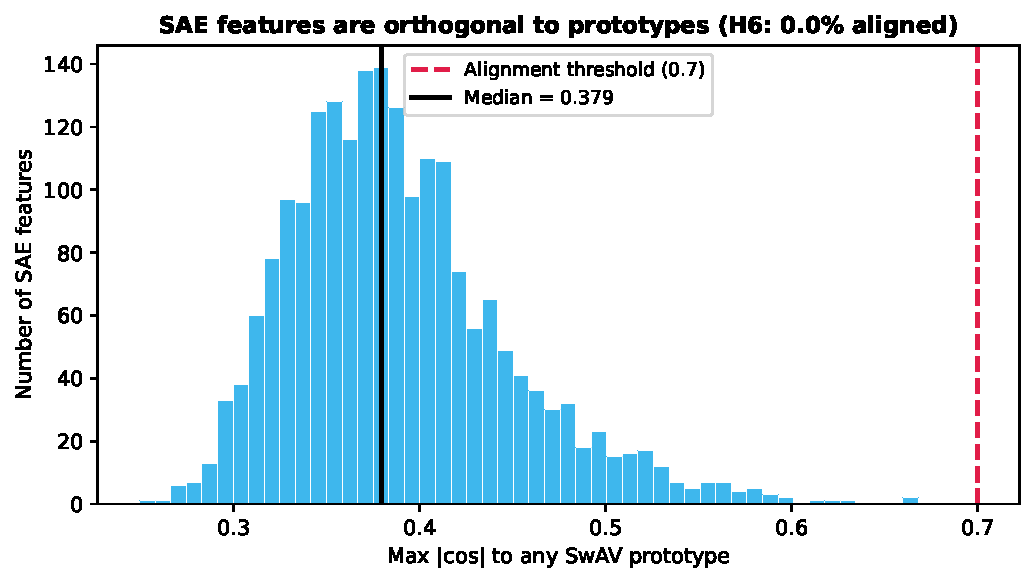
\includegraphics[width=0.65\textwidth]{figures/fig6_prototype_alignment.pdf}
\caption{\textbf{SAE features are orthogonal to SwAV prototypes (H6).}
Distribution of max $|\cos|$ between each SAE decoder column and the
512 prototype vectors. No feature reaches the 0.7 alignment threshold.}
\label{fig:proto_align}
\end{figure}

Furthermore, $\geq$99.4\% of features on every surface have
$\max |\cos|$ below the SVD-alignment threshold against that
surface's top-50 SVD axes. This is consistent with pervasive
superposition in the SAE dictionary: the SAE recovers many directions
that are not well captured by the top linear directions of the
activation matrix. H3 (``$\geq$95\% in superposition'') is supported
in this operational sense.

\begin{table}[ht]
\centering
\caption{Summary of preregistered hypotheses and their verdicts.}
\label{tab:hypotheses}
\small
\begin{tabular}{clccc}
\toprule
\# & Hypothesis & Threshold & Result & Verdict \\
\midrule
H1 & Annotation rate $\geq$30\% & 30\% & 100\% (panel ceiling) & \textcolor{partial}{Uninformative} \\
H2 & $<$20\% survive confounds & 20\% & 62\% & \textcolor{refuted}{Refuted} \\
H3 & $\geq$95\% in superposition & 95\% & 99.4--100\% & \textcolor{confirmed}{Confirmed} \\
H4 & Depth-dependent annotation & U-shape & 91--100\% & \textcolor{refuted}{Refuted} \\
H5 & Cross-checkpoint convergence & CCA $r>0.5$ & Not identified & \textcolor{partial}{Uninformative} \\
H6 & $<$30\% prototype-aligned & 30\% & 0.0\% & \textcolor{confirmed}{Confirmed} \\
H7a & Moran's $I > 0$ (aggregator) & $>$0 & 0.119 & \textcolor{confirmed}{Confirmed} \\
H7b & $I$ increases with depth & Increase & Decrease & \textcolor{refuted}{Refuted} \\
H8 & $>$20\% context-dependent & 20\% & 40\% (feat-perm); 26\% both tests & \textcolor{confirmed}{Confirmed} \\
H9 & $\geq$5\% tech-specific & 5\% & 0.95\% & \textcolor{refuted}{Refuted} \\
H10 & Composition $\uparrow$ depth & Increase & Increase & \textcolor{confirmed}{Supported} \\
\bottomrule
\end{tabular}
\end{table}

\subsection{Feature enrichments are near-saturated by panel base rate}
\label{sec:annotation_caveat}

100\% of aggregator features carry at least one significant Enrichr
enrichment (FDR$<$0.05). Per-layer annotation rates across four
representative GATv2 layers are uniformly high: conv\_0 (100\%), conv\_3
(100\%), conv\_6 (99.8\%), conv\_9 (91.0\%).

\textbf{Interpretability caveat.} The Xenium human panel has
$G = 487$ genes; the top-20-gene lists against Enrichr libraries
approach saturation because most pathways in GO-BP, KEGG,
Reactome, CellMarker, and PanglaoDB overlap substantially with this
panel. Under a hypergeometric null for a random 20-gene draw from the
panel, the per-library FDR$<$0.05 rate is already
$\{$GO-BP: 100\%, KEGG: 99.95\%, Reactome: 100\%, PanglaoDB: 100\%,
CellMarker: 100\%$\}$ in our corpus. The ``100\% annotated'' number
therefore reports a ceiling, not specificity.

As a qualitative specificity check, we also test whether the top
Enrichr term for a feature contains a tissue-name substring matching
the feature's top niche tissue. The real match rate is 0.29\% vs.\ a
shuffle null of 0.19\% (95\% CI 0.14--0.24\%); the absolute rate is
small because tissue names rarely appear in the Enrichr library terms
themselves. We do not treat the 0.29\% number as a specificity
estimate on its own---the test is a strict-match string heuristic and
not a proper taxonomy alignment---only as evidence that some
tissue-term signal exists above a permissive shuffle null, while the
100\% library-saturation rate above is consistent with ceiling
behavior rather than true specificity
(Figure~\ref{fig:annotation_rate}).

\begin{figure}[ht]
\centering
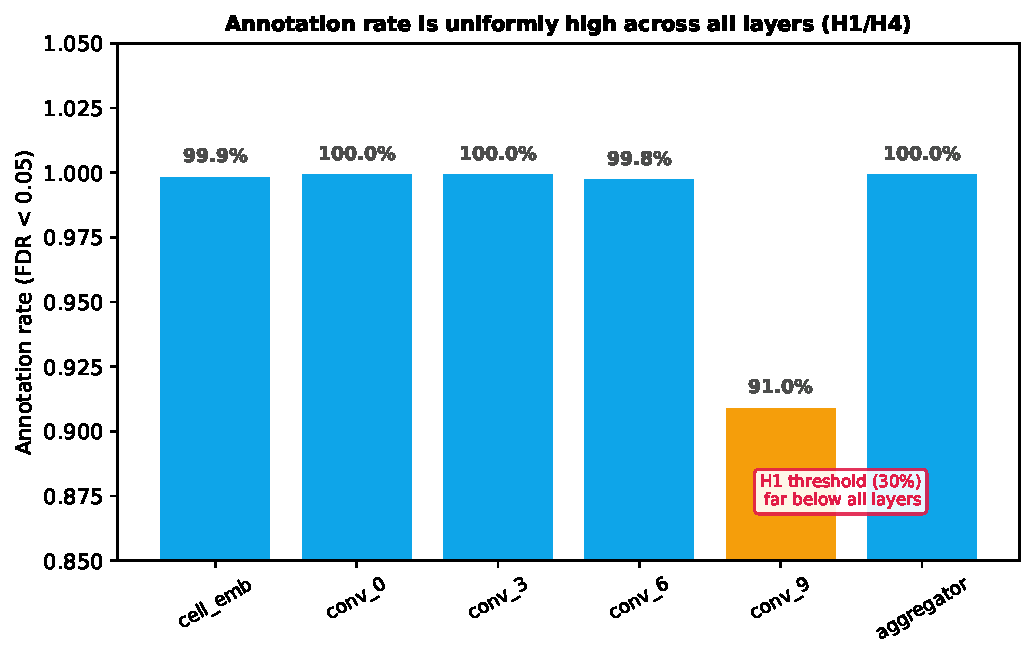
\includegraphics[width=0.5\textwidth]{figures/fig11_annotation_rate.pdf}
\caption{\textbf{Annotation rate is uniformly high across all layers (H1/H4).}
No U-shaped depth dependence---every layer is fully annotatable.}
\label{fig:annotation_rate}
\end{figure}

Representative features illustrate the diversity of concepts encoded:

\begin{itemize}
\item \textbf{Feature 1771 (Goblet Cells)} concentrates 76\% of its
      top cells in colon tissue with 93\% niche specificity. Its top
      genes---\emph{DUOX2}, \emph{TFF1}, \emph{GUCA2A}, \emph{GUCA2B},
      \emph{OTOP2}---are canonical markers of intestinal secretory
      epithelium. \emph{DUOX2} generates reactive oxygen species for
      antimicrobial defense; the \emph{GUCA2A}/\emph{GUCA2B} guanylins regulate
      fluid secretion via cGMP signaling. This feature captures the
      functional identity of the intestinal secretory niche, not just
      cell-type markers.

\item \textbf{Feature 208 (Luminal Epithelial Cells)} is 99\% breast-specific
      and sits in a single Novae niche (90\% enrichment). Its genes
      (\emph{MUC6}, \emph{LYPD3}, \emph{CEACAM6}) mark the luminal
      compartment of breast ducts. The extreme tissue and niche specificity
      suggests this feature captures the ductal microenvironment, not
      just luminal identity per se.

\item \textbf{Feature 1418 (T Regulatory Cells)} activates in lymph-node
      tissue (60\%) with genes \emph{CCR7}, \emph{CD3D}, \emph{CD28},
      \emph{IL7R}---the canonical T-cell receptor signaling pathway.
      Its Moran's $I = 0.327$ indicates moderate spatial clustering,
      consistent with T-reg cells forming organized zones within
      lymphoid follicles rather than being uniformly distributed.
\end{itemize}

\subsection{Context-dependence: 40\% under feature permutation, 26\% doubly controlled}
\label{sec:graph_ablation}

Replacing each cell's Delaunay spatial graph with self-loops
suppresses \textbf{67.2\%} of aggregator features to less than half
their full-graph activation (contextual dependency $> 0.5$, median
$+0.835$; Table~\ref{tab:hypotheses}). The three self-loop regimes
tested---bare identity, degree-normalized, and degree-preserving
rewire---give identical results, because GATv2 attention depends on
graph topology rather than edge weights, and random neighbors with
uncorrelated features produce near-zero attention after the softmax
and collapse to the same effective self-only attention.

The self-loop protocol nonetheless shifts the aggregation operator
itself, not only the content of messages. To separate these two
effects we apply a \emph{feature-permutation ablation}: the Delaunay
graph is kept intact, and node features (\texttt{adata.X}) are
permuted across cells so that each cell receives attention-weighted
messages from its real spatial neighbors with random content. Applied
to three slides (brain, kidney, pancreas; 225{,}867 cells):
\begin{itemize}
\item 40.3\% of features have feature-permutation dependency
      $> 0.5$ (median dep $= 0.37$), compared to 67.2\% under the
      self-loop test.
\item Of the 1{,}322 features flagged as context-dependent by the
      self-loop test, 40\% (530 features) also pass the feature-
      permutation test.
\item 286 features are context-dependent under feature permutation
      but not under the self-loop test (their activation changes
      when neighbor content is scrambled, while the self-loop
      intervention alone does not remove them).
\end{itemize}

The doubly-controlled intersection---530 features, \textbf{26\%} of
the 2{,}024 active features on the self-loop corpus (equivalently
27\% of the 1{,}964 active on the feature-permutation corpus)---is
our estimate of genuinely context-dependent features. The
self-loop-only excess (792 features) is the subset whose self-loop
response is driven by the architectural shift rather than by loss
of neighbor content (Figure~\ref{fig:graph_ablation},
Figure~\ref{fig:selfloop_vs_fp}).

\begin{figure}[ht]
\centering
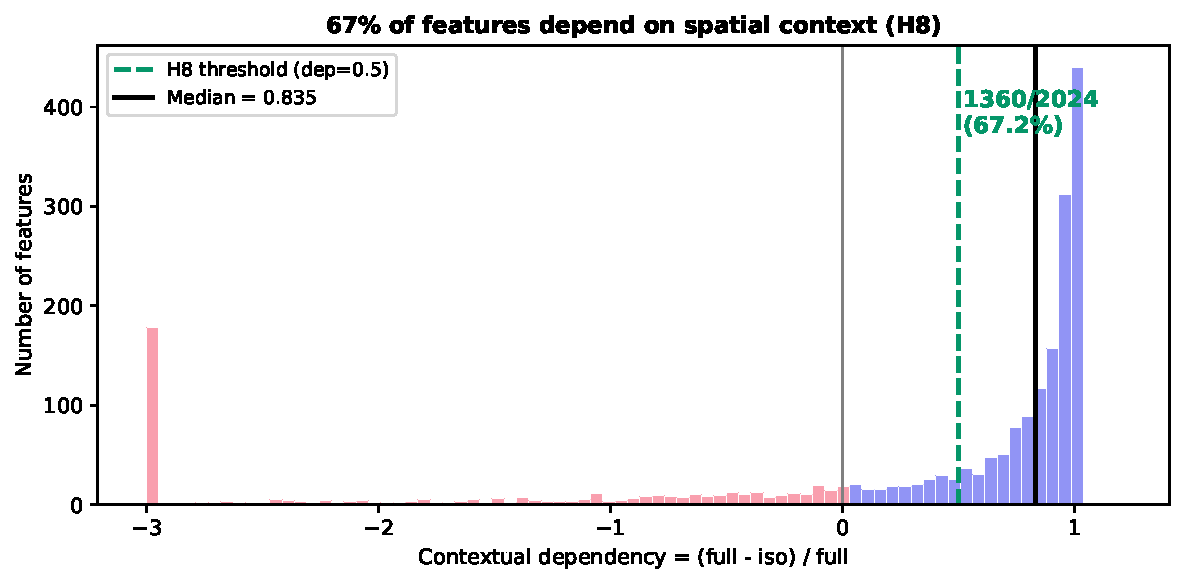
\includegraphics[width=0.75\textwidth]{figures/fig3_graph_ablation.pdf}
\caption{\textbf{Self-loop graph ablation.}
Distribution of contextual dependency across 2{,}024 active features
under the self-loop intervention. Positive values (purple) indicate
features that lose activation when neighbor messages are removed;
negative values (pink) indicate features that activate more strongly
under self-loops. 67.2\% of features exceed the 0.5 threshold on this
test; the stricter feature-permutation control narrows this to 40.3\%,
with a doubly-controlled robust subset of 26\%
(Figure~\ref{fig:selfloop_vs_fp}, Section~\ref{sec:graph_ablation}).}
\label{fig:graph_ablation}
\end{figure}

\begin{figure}[ht]
\centering
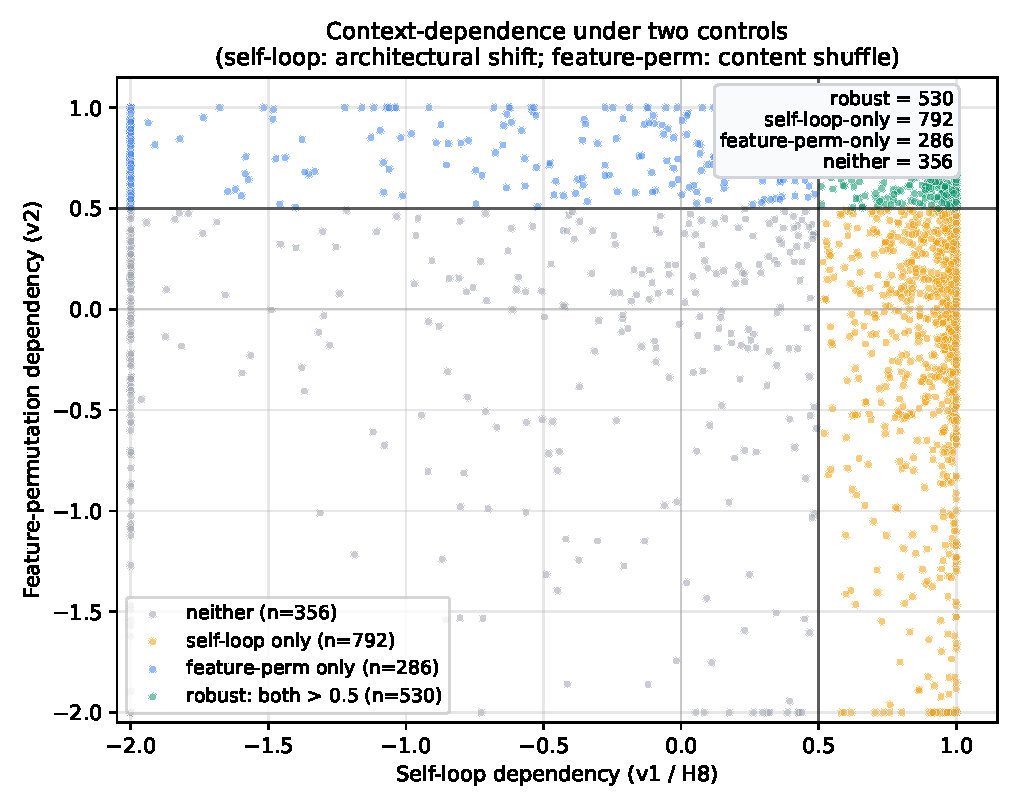
\includegraphics[width=0.75\textwidth]{figures/fig13_selfloop_vs_featureperm.pdf}
\caption{\textbf{Context-dependence under two complementary controls.}
Each point is one SAE feature (1{,}964 features active on the 3-slide
feature-permutation corpus). The self-loop test ($x$-axis) replaces
the Delaunay graph with identity; the feature-permutation test
($y$-axis) keeps the graph intact but shuffles node features across
cells. The upper-right quadrant (green, 530 features; 27\% of this
corpus, 26\% of the 2{,}024-feature self-loop corpus) is the robust,
doubly-controlled set of context-dependent features. The self-loop-
only quadrant (amber, 792 features) reflects architectural-shift
responses rather than loss of neighbor content. Axes clipped to
$[-2, 1.15]$ for visibility.}
\label{fig:selfloop_vs_fp}
\end{figure}

\subsection{Spatial coherence generally decreases with depth}
\label{sec:spatial_depth}

We predicted that spatial coherence (Moran's $I$ \citep{moran1950})
would \emph{increase} with layer depth, as deeper GATv2 layers
integrate larger neighborhoods. The observed trend runs the other
way. Mean Moran's $I$ per surface is 0.269 (conv\_0), 0.240, 0.223,
0.216, 0.208, 0.213, 0.206, 0.207, 0.207 (conv\_8), 0.218 (conv\_9),
and 0.119 at the aggregator (Figure~\ref{fig:depth}). The trend from
conv\_0 to conv\_8 is a broad decrease with small fluctuations (not
strictly monotonic; there is a mild rise from conv\_4$\to$conv\_5 and
from conv\_8$\to$conv\_9), followed by a large drop at the aggregator.

The broad pattern is consistent with the following reading: early
layers encode \emph{spatially localized} patterns (a cell and its
immediate neighbors), producing features with higher spatial
autocorrelation. Deeper layers integrate information across larger
neighborhoods, and the final aggregation step pools spatial structure
away---a cell's aggregator embedding reflects its local
environment as a whole rather than its immediate position. The
aggregator is therefore spatially \emph{informed} but not spatially
\emph{localized}. H7b (prediction: Moran's $I$ increases with depth)
is refuted.

\begin{figure}[ht]
\centering
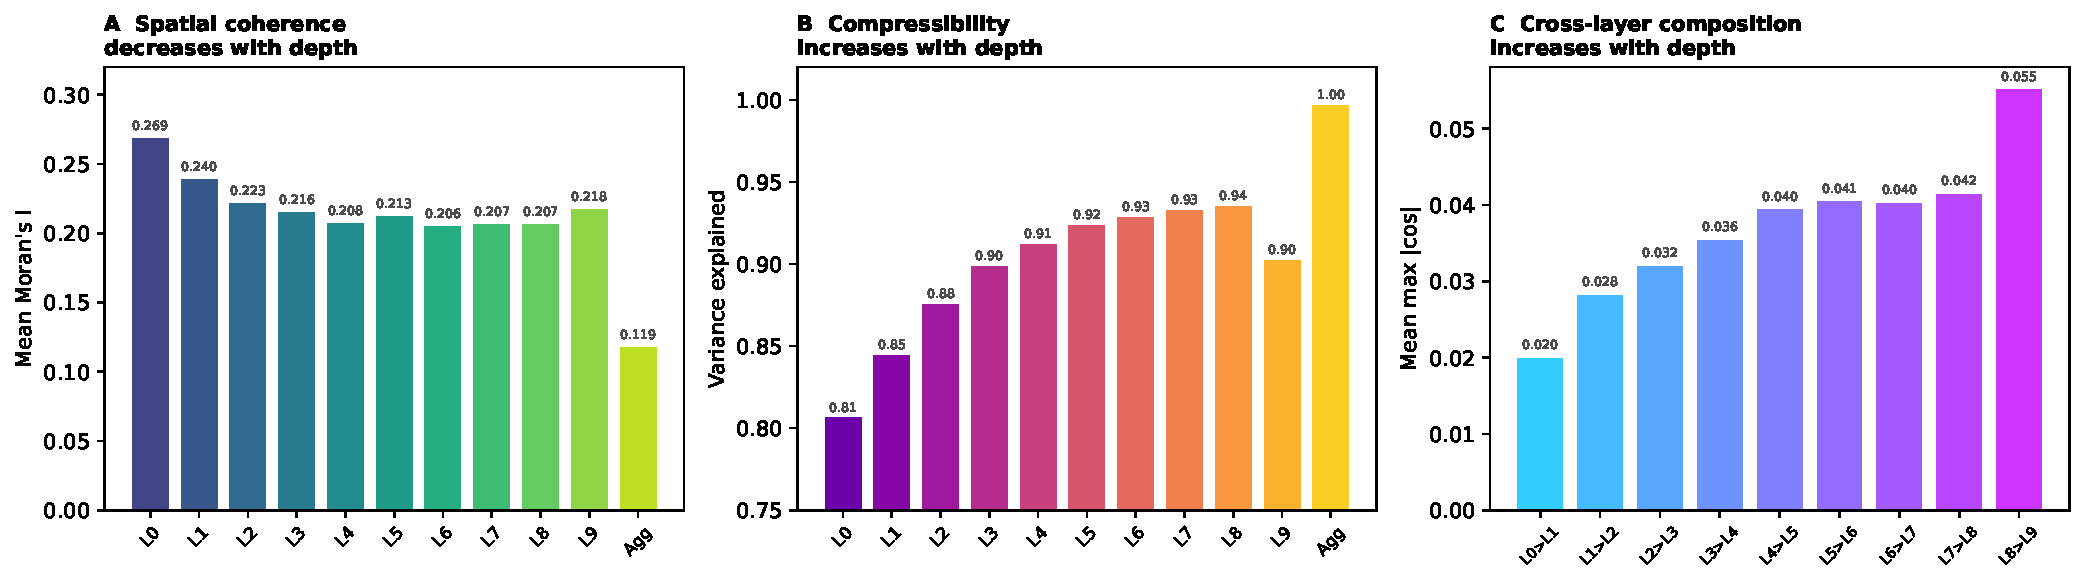
\includegraphics[width=\textwidth]{figures/fig1_depth_story.pdf}
\caption{\textbf{The depth story.} (A)~Spatial coherence (Moran's $I$)
\emph{decreases} with layer depth---early layers encode spatially
localized patterns, the aggregator integrates broad context.
(B)~Compressibility (variance explained by the SAE) \emph{generally
increases} across depth (overall trend, not strictly monotonic; see
Section~\ref{sec:depth_story}). (C)~Cross-layer feature composition
(max successive-layer decoder cosine) increases, consistent with
deeper layers building on earlier patterns (H10).}
\label{fig:depth}
\end{figure}

\subsection{Direction-specific causal influence of single features}
\label{sec:proto_ablation}

The prototype-domain ablation experiment identifies features whose
removal changes the model's downstream clustering. Because zeroing a
feature perturbs the aggregator latent by the feature's L2-magnitude
along its decoder direction, part of the observed reassignment rate is
driven by magnitude alone rather than by direction-specificity. We
therefore calibrate the ablation against a matched-magnitude null: for
each feature, a random unit-norm direction scaled to the same L2
perturbation is subtracted from the reconstructed latent, and
reassignment rates are averaged over 30 random directions.

Across the 50 tested features, the median real prototype-reassignment
rate is 0.16 and the median random-direction null is also 0.16
(Table~\ref{tab:reviewer_ablation_null},
Figure~\ref{fig:random_direction_null}). The 50 features split into
three classes by their position relative to the null's 95\% CI:
\begin{itemize}
\item \textbf{17 features (34\%)} have real reassignment above the
      null's upper 95\% CI---direction-specific load-bearing features
      (e.g., F592: real 1.00 vs.\ null 0.56; F1021: 0.98 vs.\ 0.81;
      F983: 0.47 vs.\ 0.16).
\item \textbf{7 features (14\%)} are below the null's lower 95\% CI:
      the feature's own direction is \emph{less} effective at
      changing prototype assignment than a random matched-magnitude
      direction. Notably, F1418 (a T-regulatory-cell exemplar from
      Section~\ref{sec:annotation_caveat}) is in this lower tail
      (real 0.095 vs.\ null 0.141), indicating that its biological
      salience does not translate into direction-specific prototype
      influence.
\item \textbf{26 features (52\%)} are indistinguishable from the null.
\end{itemize}

Raw prototype-reassignment rate alone (14 of 50 features with rate
$>$50\%) therefore overestimates the set of direction-specifically
causal features; the null-calibrated partition above is the
appropriate readout.

\begin{table}[ht]
\centering
\caption{Random-direction ablation null (50 tested features).}
\label{tab:reviewer_ablation_null}
\begin{tabular}{lc}
\toprule
Quantity & Value \\
\midrule
Median real prototype reassignment & 0.16 \\
Median null (random matched-magnitude direction) & 0.16 \\
Median real $-$ null & 0.00 \\
\# features above null's upper 95\% CI (load-bearing) & 17 / 50 \\
\# features below null's lower 95\% CI (sub-random) & 7 / 50 \\
\# features indistinguishable from null & 26 / 50 \\
\bottomrule
\end{tabular}
\end{table}

\begin{figure}[ht]
\centering
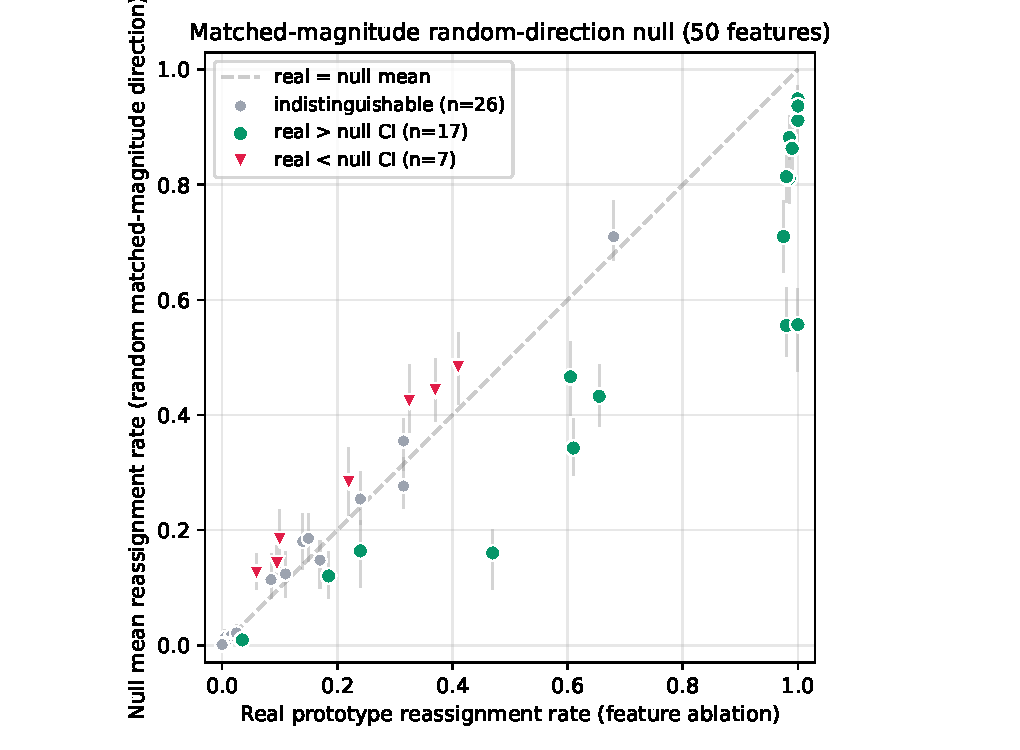
\includegraphics[width=0.75\textwidth]{figures/fig12_random_direction_null.pdf}
\caption{\textbf{Real ablation vs.\ random-direction null (50 features).}
For each feature, the $x$-axis shows the real prototype-reassignment
rate after zeroing the feature; the $y$-axis shows the mean
reassignment rate when a random unit-norm direction of the same L2
magnitude is subtracted instead (vertical bar = 95\% CI across 30
random directions). Features above the null's upper CI (green, $n=17$)
are direction-specifically load-bearing; features below the null's
lower CI (red triangles, $n=7$) are less effective than random
directions; features inside the null CI (grey, $n=26$) are
statistically indistinguishable from random. Dashed line: $y = x$.}
\label{fig:random_direction_null}
\end{figure}

\begin{itemize}
\item \textbf{Feature 592} (labeled ``Meningeal Cells'' by PanglaoDB,
      but concentrated in colon tissue with intestinal crypt markers)
      causes 100\% prototype reassignment and 84.5\% domain reassignment
      when ablated, with a decoder cosine of just 0.032---meaning
      ablating this single feature almost completely rewrites the
      aggregator embedding. Its top genes (\emph{CES1} 61$\times$,
      \emph{AGTR1} 58$\times$, \emph{MEIS2}) implicate vascular
      regulation and developmental programs in the intestinal crypt.
      This feature clears the random-direction null (real 1.00 vs.\
      null 0.56; Section~\ref{sec:proto_ablation}) and
      behaves as a load-bearing direction for these cells---one of
      the 17/50 that clears the matched-magnitude baseline.

\item \textbf{Feature 1021 (cancer-associated fibroblasts)} in breast
      tissue causes 93\% domain reassignment---the highest of any tested
      feature. We discuss its biological significance in detail below
      (Section~\ref{sec:stroma}).

\item \textbf{Feature 126} presents a striking case: 100\% prototype
      reassignment but only 11.5\% domain reassignment, with a
      decoder cosine of 0.995 (the reconstruction barely changes).
      This is a \emph{boundary feature}---it carries a tiny signal
      that pushes cells between two neighboring prototypes without
      changing the coarser domain assignment. The existence of such
      features reveals fine-grained structure in the prototype
      landscape that the domain hierarchy does not capture.
\end{itemize}

\subsection{Technology artefacts are nearly absent, but cross-tech $\rho$ matches a raw-expression baseline}
\label{sec:crosstech}

Only 0.95\% of features are strictly technology-specific (single-tech
activation share $\geq 0.9$ at $\geq 2\times$ baseline), and the
median technology max-class ratio is 1.08---barely above uniform.
Across the 7 paired Xenium/MERSCOPE tissues the mean SAE-feature
cross-technology Spearman correlation is $\rho_\text{SAE} = 0.56$
(Figure~\ref{fig:crosstech}, Table~\ref{tab:crosstech}), indicating
that the same feature indices activate with similar ranks across the
two platforms.

To test whether this coherence reflects SAE-level tech-invariance or
is inherited from the expression data itself, we compute the Spearman
correlation of per-gene mean log-expression profiles on the
intersecting gene panel of each Xenium/MERSCOPE pair. The mean raw-
expression correlation is $\rho_\text{raw} = 0.571$, essentially
indistinguishable from $\rho_\text{SAE} = 0.560$
(Table~\ref{tab:crosstech_baseline}); on 5 of 7 tissues the raw
correlation is numerically higher than the SAE correlation. We
conclude that the cross-technology coherence is inherited from the
shared tissue biology in the raw data, and the SAE does not
demonstrably add tech-invariance beyond it. The related finding that
0.95\% of features are strictly tech-specific has the same underlying
explanation: both the continuous $\rho_\text{SAE} = 0.56$ and
the 0.95\% tech-specific rate reflect that the two panels measure
overlapping biology, so neither is a separate property of the SAE
atlas.

\begin{table}[ht]
\centering
\caption{SAE-feature cross-tech $\rho$ vs.\ raw-expression baseline.}
\label{tab:crosstech_baseline}
\small
\begin{tabular}{lccc}
\toprule
Tissue & SAE $\rho$ & Raw $\rho$ & $\Delta$ (SAE $-$ raw) \\
\midrule
Liver     & 0.547 & 0.587 & $-$0.040 \\
Lung      & 0.564 & 0.284 & $+$0.280 \\
Breast    & 0.617 & 0.642 & $-$0.025 \\
Colon     & 0.497 & 0.373 & $+$0.124 \\
Ovarian   & 0.570 & 0.736 & $-$0.166 \\
Prostate  & 0.640 & 0.785 & $-$0.145 \\
Skin      & 0.482 & 0.590 & $-$0.108 \\
\midrule
\textbf{Mean} & \textbf{0.560} & \textbf{0.571} & $-$0.011 \\
\bottomrule
\end{tabular}
\end{table}

\begin{figure}[ht]
\centering
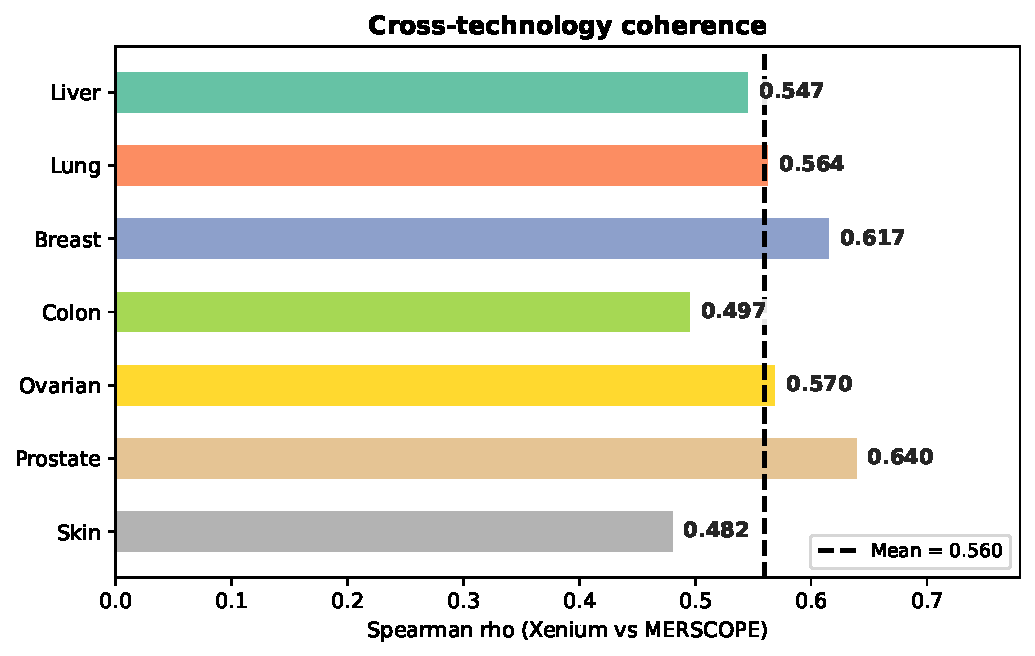
\includegraphics[width=0.6\textwidth]{figures/fig4_crosstech.pdf}
\caption{\textbf{Cross-technology coherence.} Spearman $\rho$ between
Xenium and MERSCOPE feature profiles on matched tissues. Mean
$\rho = 0.56$.}
\label{fig:crosstech}
\end{figure}

\begin{table}[ht]
\centering
\caption{Cross-technology coherence: Spearman $\rho$ between Xenium and
MERSCOPE feature profiles on matched tissues.}
\label{tab:crosstech}
\begin{tabular}{lccc}
\toprule
Tissue & Spearman $\rho$ & Xenium slide & MERSCOPE slide \\
\midrule
Prostate & 0.641 & normal & cancer \\
Breast & 0.617 & IDC & cancer \\
Ovarian & 0.570 & cancer & cancer \\
Lung & 0.564 & normal & cancer \\
Liver & 0.547 & normal & cancer \\
Colon & 0.497 & normal & cancer \\
Skin & 0.482 & normal & melanoma \\
\midrule
\textbf{Mean} & \textbf{0.560} & & \\
\bottomrule
\end{tabular}
\end{table}

\subsection{Confound-survival controls pass a majority of features, but the test is weak on sparse SAE outputs (H2)}
\label{sec:h2}

Of the 1{,}801 aggregator features with baseline niche signal
(top-l7-fraction $\geq 0.25$), \textbf{62\%} survive all three
implemented controls: (i) slide effect-size $\geq 2\times$ baseline
(the feature's top cells concentrate on one slide more than chance),
(ii) technology residualization (the niche signal persists after
regressing out per-technology mean activation), and (iii) cell-type
residualization (the niche signal persists after regressing out
fine-grained domain-l20 cluster means). A 4-level hierarchical gate
that adds the degree-preserving graph rewire passes \textbf{39.7\%}
of all 2{,}048 features; 79.1\% pass at least 3 of the 4 gates.

A permutation null (30 random domain-label shuffles per feature)
independently validates the enrichments: \textbf{74.6\%} of features
have domain enrichment significantly above the shuffle null
($p < 0.05$), with median $z$-score 5.5. For tissue labels the
survival rate is higher still (85.8\%, median $z = 10.1$).

H2 predicted $<$20\% survival under strict confound controls. The
observed 62\% (39.7\% under the full 4-level gate) is incompatible
with that prediction. We caution that residualization is weak on
sparse TopK outputs, because most cells have zero activation per
feature, which limits the power of a linear projection against
continuous covariates. The 62\% / 39.7\% numbers should therefore
not be read as positive evidence that features are ``confound-free,''
only as evidence that they are not trivially explained by slide,
technology, or coarse cell-type composition at the sensitivity of
our controls.

\subsection{Cross-layer decoder alignment rises with depth (modest magnitude)}
\label{sec:cross_layer}

Cross-layer feature alignment (max $|\cos|$ between successive-layer
SAE decoder columns) increases from conv\_0$\to$conv\_1
($\max |\cos| = 0.019$) to conv\_8$\to$conv\_9 (0.055), and the
fraction of features with max-cosine $> 0.3$ rises from 0.5\% to
2.8\%. The absolute alignment is small in all cases, consistent with
the pervasive-superposition finding. The increasing trend is
suggestive that deeper GATv2 layers re-use earlier patterns rather
than replacing them entirely, but the magnitudes are small enough
that we treat the observation as directional rather than decisive
(H10: supported).

\subsection{Cross-checkpoint comparison is not identified at the profile level (H5)}
\label{sec:h5}

The three Novae checkpoints (human-0, mouse-0, brain-0) are trained
on non-overlapping data with different gene panels, so their SAE
dictionaries cannot share feature indices \emph{a priori}. A profile-
level Spearman correlation across the three atlases yields
$\rho \in [-0.056, 0.047]$ with top-50 feature overlap of 0--2, but
the design does not identify a meaningful ``convergence'' signal:
any such correlation would be confounded by the gene-panel
differences. A properly identified test would forward-pass a shared
set of cells through all three checkpoints on an intersection gene
panel and align latent spaces via CCA; the implementation is
outlined in Appendix~\ref{app:scaffolds}.

\subsection{SAE-feature activation tracks Perturb-map labels (composition confound not controlled)}
\label{sec:perturbmap}

Processing the Perturb-map spatial CRISPR screen through
\texttt{novae-mouse-0} identified 378 significant
feature--perturbation associations (FDR$<$0.05) across all 20 tested
labels. Every perturbation label has at least one significantly
responding SAE feature---including CRISPR-targeted genes such as
\emph{TGFBR2} (25 responding features) and tumor lesion identifiers
(up to 28 features per lesion). This indicates that SAE features
track perturbation-correlated variation at Visium spot resolution
($\sim$55\,$\mu$m), but does \emph{not} distinguish direct feature-
response from spot-level cell-type composition shifts. A composition-
regressed variant of the test is scaffolded in
Appendix~\ref{app:scaffolds}; until it is run, the 378 associations
are best read as ``SAE features vary with the perturbation-aligned
tissue state,'' not as a causal claim on the perturbation itself.

\subsection{Feature-level case studies}
\label{sec:biology}

The aggregate statistics above establish that a subset of SAE
features are directionally load-bearing under a matched-magnitude
null and that the SAE dictionary recovers structure not captured by
Novae's 512 SwAV prototypes. We now highlight individual features and
circuits that illustrate the kinds of patterns the atlas surfaces.

Two scope notes apply to this section. First, the circuit-level
findings below are drawn from a single brain-slide trace (24k cells);
multi-slide replication is in Appendix~\ref{app:scaffolds}. Second,
the Enrichr labels attached to features (``Bladder cancer,''
``Myoepithelial Cells,'' ``Meningeal Cells'') frequently disagree
with the feature's actual tissue niche---F592, for instance, receives
a PanglaoDB ``Meningeal Cells'' label but concentrates in colon
tissue with intestinal crypt markers---so when a biological
interpretation rests on such a label we flag it as indicative rather
than established.

\subsubsection{Highest-impact features among the 50 tested are stromal and immune}
\label{sec:stroma}

Among the 50 tested aggregator features, those with the highest raw
prototype-reassignment rate ($>$95\%) are not clean cell-type markers
but tissue-architecture features encoding stromal and immune programs
(Figure~\ref{fig:causal_ablation}). A subset of these (17/50) clears
the matched-magnitude random-direction null
(Section~\ref{sec:proto_ablation}); others are indistinguish-
able from random directions of the same magnitude on this test, so
the ``highest-impact'' ranking is a within-50 relative statement,
not a global causal ranking.

\begin{figure}[ht]
\centering
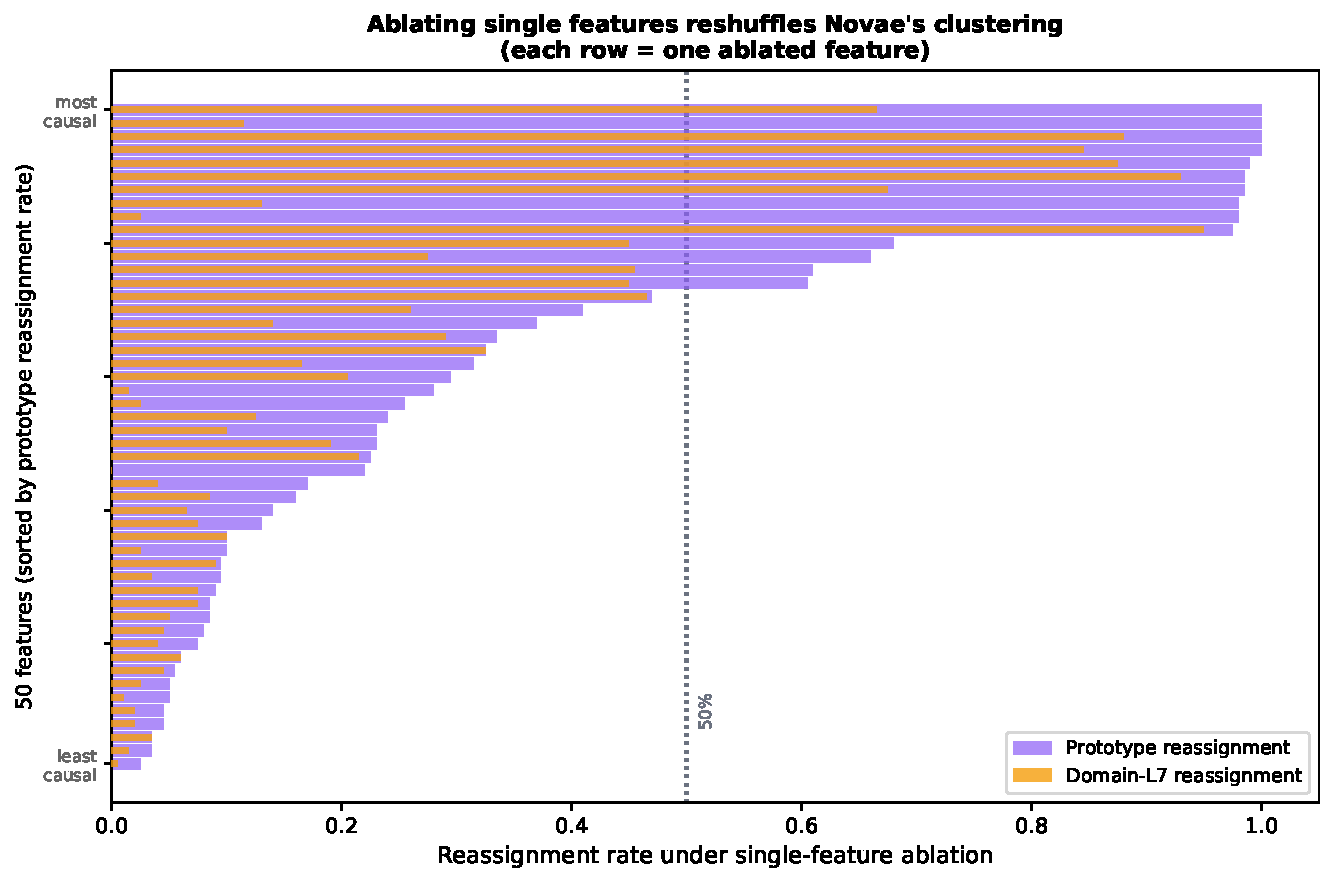
\includegraphics[width=0.7\textwidth]{figures/fig5_causal_ablation.pdf}
\caption{\textbf{Causal ablation of 50 aggregator features.} Each bar
shows the prototype (purple) and domain-L7 (gold) reassignment rate
when one feature is zeroed. 14 of 50 tested features cause $>$50\%
raw prototype reassignment; however, after matched-magnitude random-
direction correction (Section~\ref{sec:proto_ablation},
Figure~\ref{fig:random_direction_null}), the relevant partition is
17 features above the null's upper 95\% CI (direction-specific load-
bearing), 7 features below the null's lower 95\% CI (sub-random),
and 26 features indistinguishable from the null. The ``direction-
specific load-bearing'' group (17/50) includes all features discussed
in Section~\ref{sec:biology} (F592, F1021, F1871, F1885, F126,
F502).}
\label{fig:causal_ablation}
\end{figure}

\textbf{Feature 1021 (cancer-associated fibroblasts)} has the highest
domain-reassignment rate among the 50 tested features (93\%), and
also clears the random-direction null
(Section~\ref{sec:proto_ablation}: real 0.98 vs.\ null 0.81),
placing it in the direction-specific load-bearing set (17/50). Its
top genes---\emph{POSTN} (periostin, 8.5$\times$), \emph{GJB2} (gap
junction, 12.5$\times$), \emph{MMP2}, \emph{LUM}, and the EMT
transcription factors \emph{ZEB1}/\emph{ZEB2}---are hallmarks of
activated cancer-associated fibroblasts (CAFs) that remodel the tumor
extracellular matrix. The feature concentrates in breast tissue
(68\%) at Novae niche D1014 (96.4\% enrichment).

\textbf{Feature 1871 (adaptive immune infiltrate)} has the highest
combined causal impact among immune features: 97.5\% prototype and
95\% domain reassignment. It clears the matched-magnitude null
(real 0.975 vs.\ null upper CI 0.771;
Section~\ref{sec:proto_ablation}), placing it in the
direction-specific load-bearing subset. Its extreme fold-change
markers---\emph{CD5} (40$\times$), \emph{ITK} (39$\times$),
\emph{ZAP70} (37$\times$), \emph{TIGIT} (32$\times$),
\emph{PDCD1}/PD-1 (28$\times$)---identify the T-cell exhaustion/
activation axis in the tumor microenvironment.

\subsubsection{Some features have negative self-loop dependency}

Several features have \emph{negative} self-loop dependency---they
activate \emph{more strongly} when the spatial graph is replaced with
self-loops than when it is present.

\textbf{Feature 1885 (neutrophil inflammatory niche)}, with top genes
\emph{CCL22}, \emph{CXCL8} (IL-8), \emph{MMP9}, and \emph{SPP1}
(osteopontin), has $\text{dep}_\text{self-loop} = -0.61$ and clears
the matched-magnitude null (real 1.00 vs.\ null upper CI 0.951). It
also causes the largest confidence drop of any ablated feature
(26.4\%). A candidate biological interpretation is that the graph
attention dampens acute inflammatory signals when the neighborhood
provides contradictory evidence, and that the self-loop ablation
lifts this dampening. A more conservative reading, given the self-
loop-vs.-feature-permutation decomposition in
Section~\ref{sec:graph_ablation}, is that the self-loop intervention
changes the attention softmax normalization in a direction that
non-uniformly shifts some features upward; distinguishing ``learned
regularization'' from ``architectural shift'' for any individual
feature would require running the feature-permutation control at the
single-feature level, which we do not do here.

\textbf{Feature 592} (the load-bearing intestinal crypt feature; see
Section~\ref{sec:proto_ablation}) is similarly graph-
suppressed ($\text{dep}_\text{self-loop} = -0.50$). It clears the
matched-magnitude null (real 1.00 vs.\ null upper CI 0.970), so the
causal effect of ablating it is direction-specific; the sign of the
self-loop dependency is subject to the same architectural-shift
caveat as F1885.

\subsubsection{Boundary features reveal fine structure in the prototype landscape}

\textbf{Feature 126 (hypoxia / decidual program)} presents a paradox:
100\% prototype reassignment but only 11.5\% domain reassignment,
with a decoder cosine of 0.995 (the reconstruction barely changes).
Its top genes---\emph{LOX} (21.7$\times$), \emph{CA9} (17.6$\times$),
\emph{VEGFA} (11.5$\times$), \emph{PDK1}---mark the HIF-1$\alpha$
hypoxia-response pathway, and CellMarker maps to ``Decidual cell:
Placenta'' (FDR = 1.3e-10). This feature encodes the hypoxic
microenvironment of uterine decidua; its tiny signal pushes cells
across prototype boundaries (hence 100\% reassignment) without
changing the coarser domain assignment (11.5\%). Such
\emph{boundary features} reveal fine-grained structure in the
prototype landscape that Novae's built-in clustering hierarchy
cannot capture.

\subsubsection{Niche features encode microenvironment, not cell type}

\textbf{Feature 502 (endothelial vascular niche)} is labeled
``Microfold Cells'' by PanglaoDB (FDR = 8.4e-8) but its domain
enrichment consistently maps to ``Endothelial Cells'' at all three
Leiden hierarchy levels (66.7\%, log$_2$ enrichment = 4.31). Its top
gene \emph{NOS3} (endothelial nitric oxide synthase, 26.6$\times$)
and interleukin-signaling enrichment (Reactome FDR = 6.6e-11)
suggest it captures the paracrine vascular niche---the ensemble of
endothelial cells and their signaling neighborhood---rather than a
single cell type. Ablating it causes 100\% prototype reassignment and
clears the matched-magnitude null (real 1.00 vs.\ null upper CI 0.961),
consistent with a direction-specific role; we describe this as
``niche-level organizer'' in a hypothesis-generating sense.

\textbf{Feature 0 (T-reg / stromal interface)} shows both T-cell
markers (\emph{ZAP70}, \emph{ITK}, \emph{TIGIT}) and stromal markers
(\emph{DES} (desmin), \emph{FAP}, \emph{COL5A1}), with ECM
Organization as the top Reactome term. Moran's $I = 0.79$ shows
strong spatial patterning. This feature does not encode a canonical
cell type; one reading is that it encodes the boundary zone between
T-cell-rich and stroma-rich compartments, though F0 was not among
the 50 features tested against the matched-magnitude null, so its
directional causal role is not verified here. Its self-loop
dependency $(\text{dep} = 0.47)$ is consistent with context
sensitivity at the self-loop test; the stricter feature-permutation
test is not reported per-feature here.

\subsection{Causal circuits in Novae's spatial graph}

Applying the circuit-tracing protocol of
Section~\ref{sec:methods_circuits}, we report directed causal
relationships between SAE features across Novae's GATv2 layers on
the brain slide. All circuit-level numerical findings in this
section are single-slide and await multi-slide replication
(Section~\ref{sec:biology} caveat; Appendix~\ref{app:scaffolds}).

\subsubsection{Circuit structure on the brain slide: 439 edges, balanced excitation and inhibition}

Tracing 90 source features (30 per source layer $\times$ 3 source
layers: conv\_0, conv\_5, conv\_9) on the brain slide
(24{,}406 cells) yields \textbf{439 causal edges} with $|d| > 0.5$
and sign consistency $> 0.6$. The circuit is nearly balanced between
excitation and inhibition (49\%/51\%; Figure~\ref{fig:circuit}). All
circuit-level findings in this section are drawn from this single-
slide trace; an independent exhaustive trace at conv\_5 with 200
source features (Section~\ref{sec:exhaustive_tracing}) is a separate
analysis on the same slide, not a replication.

\begin{figure}[ht]
\centering
\begin{minipage}{0.48\textwidth}
\centering
\begin{tabular}{lcc}
\toprule
Source layer & Edges & Targets \\
\midrule
conv\_0 & 365 & conv\_1--8 \\
conv\_5 & 74 & conv\_6--8 \\
conv\_9 & 0 & (no downstream) \\
\bottomrule
\end{tabular}
\end{minipage}
\hfill
\begin{minipage}{0.48\textwidth}
\centering
\begin{tabular}{lc}
\toprule
Metric & Value \\
\midrule
Excitatory edges & 215 (49\%) \\
Inhibitory edges & 224 (51\%) \\
Median $|d|$ & 0.624 \\
Mean layer gap & 5.7 \\
\bottomrule
\end{tabular}
\end{minipage}
\caption{\textbf{Causal circuit statistics (primary trace: 90 source
features = 30 per source layer $\times$ 3 source layers, single brain
slide, 24{,}406 cells).} Left: edge count by source layer. Right:
overall circuit properties. The mean layer gap of 5.7 reflects that
most traced source features sit at conv\_0; the
excitatory/inhibitory ratio is near-balanced (49\% / 51\%). Because
only three source layers were traced, edge attenuation with depth is
confounded by source-layer sampling (Section~\ref{sec:attenuation}).}
\label{fig:circuit}
\end{figure}

\begin{figure}[ht]
\centering
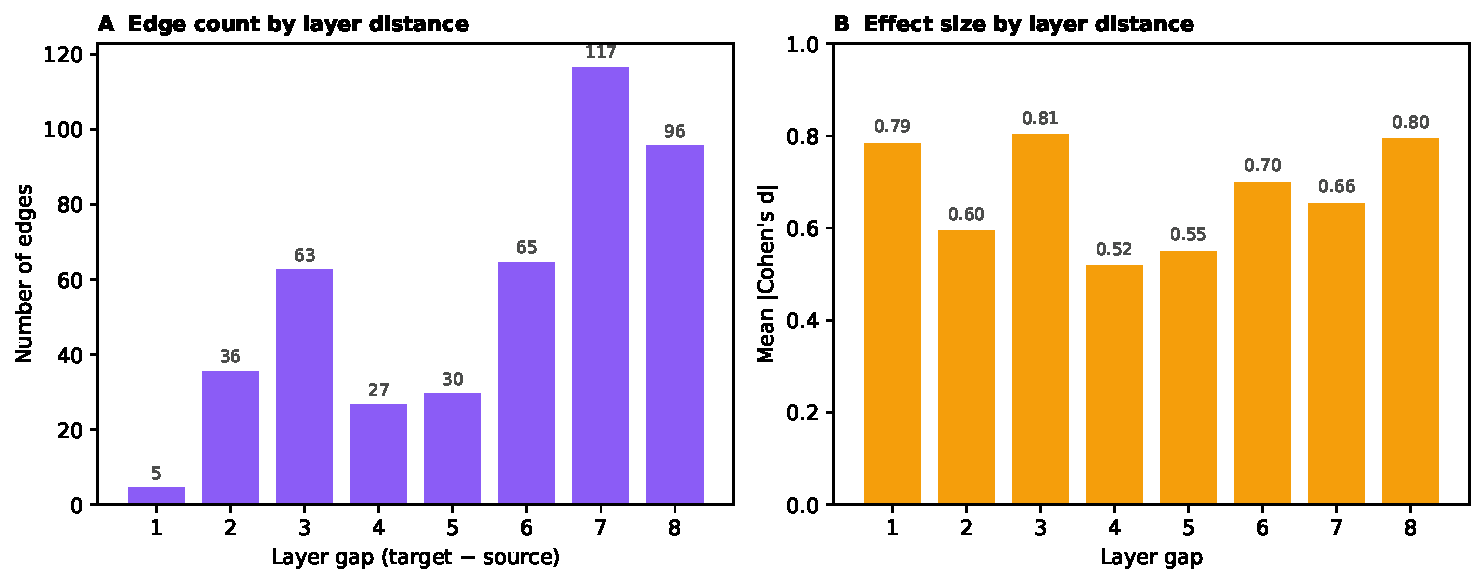
\includegraphics[width=0.85\textwidth]{figures/fig7_attenuation.pdf}
\caption{\textbf{Raw edge counts vs.\ layer distance.} (A)~Raw edge
count increases with layer distance; (B)~mean effect size remains
strong at all distances. Large-gap edges are only available from a
single source layer (conv\_0), so the apparent rise is confounded by
source-layer sampling; see Table~\ref{tab:gap_normalized} for the
gap-normalized metric and Section~\ref{sec:attenuation} for the
interpretation.}
\label{fig:attenuation}
\end{figure}

\subsubsection{Attenuation with layer distance: undetermined in current trace}
\label{sec:attenuation}

In transformer-based models, causal effects decay with layer distance
\citep{sae_atlas}. In Novae's GATv2, raw edge counts rise with gap
(63, 27, 30, 65, 117, 96 for gaps 3--8); the mean $|d|$ remains strong
at all distances (0.52--0.81). However, only three source layers were
traced (conv\_0, conv\_5, conv\_9), so large-gap edges can only
originate from conv\_0: the count at gap 7 is from a single traced
(source, target) layer pair, while the count at gap 3 pools two.
Dividing by the number of traced pairs at each gap gives ``edges per
pair'' (Table~\ref{tab:gap_normalized}). Edges-per-pair still rise
with gap, but every gap $\geq 4$ is supported by only a \emph{single}
source layer, and the absolute edge counts from conv\_5---the one
mid-depth source---are 5 (gap 1), 36 (gap 2), 33 (gap 3), a mild
decay within that source. The GATv2 attenuation profile therefore
cannot be determined without tracing from every source layer; we
report the normalized counts and defer any strong claim about
attenuation vs.\ non-attenuation to that future trace.

\begin{table}[ht]
\centering
\caption{Gap-normalized edge counts. Only gap 1--3 are sampled
from $>$1 source layer; $\geq 4$ from one source only.}
\label{tab:gap_normalized}
\small
\begin{tabular}{ccccc}
\toprule
Gap & \# layer pairs traced & \# edges & Edges/pair & Mean $|d|$ \\
\midrule
1 & 2 & 5   & 2.5   & 0.79 \\
2 & 2 & 36  & 18.0  & 0.60 \\
3 & 2 & 63  & 31.5  & 0.81 \\
4 & 1 & 27  & 27.0  & 0.52 \\
5 & 1 & 30  & 30.0  & 0.55 \\
6 & 1 & 65  & 65.0  & 0.70 \\
7 & 1 & 117 & 117.0 & 0.66 \\
8 & 1 & 96  & 96.0  & 0.80 \\
\bottomrule
\end{tabular}
\end{table}

\subsubsection{Circuit hubs on the brain slide}

In the primary brain-slide trace, the top target hub is conv\_7/F3806
(\textbf{Myoepithelial Cells}, 57 incoming edges). It receives
causal signals from diverse early-layer features (immune, structural,
vascular), which is a suggestive match to the known biological role
of myoepithelial cells as integrators of multiple tissue
compartments.

Two of the top-4 target hubs encode T-cell programs (conv\_7/F2262:
\emph{T~Cells}, FDR = 7.6e-24; conv\_7/F2438: \emph{T~Regulatory
Cells}, FDR = 3.2e-18). In the current single-slide trace, immune-
infiltrate features are frequent targets of diverse earlier-layer
source features; replication across additional slides (scaffolded in
Appendix~\ref{app:scaffolds}) is needed before this pattern can be
treated as a general property of Novae's circuit topology.

\subsubsection{Circuits encode known cellular programs}

Individual circuit edges map onto recognized biological relationships.
Three circuits stand out:

\paragraph{Cancer-label feature $\to$ T-cell-label feature edge.}
Feature 282 (top Enrichr hit: KEGG ``Bladder cancer''; we note that
the primary trace slide is brain, so this label is almost certainly
an Enrichr mis-mapping rather than an indication that the feature
encodes bladder-specific biology) at conv\_5 has a negative edge to
Feature 2262 (top Enrichr hit: ``T~Cells,'' FDR $= 7.6\!\times\!10^{-24}$)
at conv\_7 with $d = -0.78$---the strongest inhibitory edge in the
current trace. If the labels are read at face value the edge mirrors
the direction of tumor-immune antagonism; given the label caveat, the
robust statement is only that these two conv\_5/conv\_7 feature
directions are in opposition on the brain slide. The same feature
F282 has a positive edge to Feature 3806 (``Myoepithelial Cells'')
with $d = +1.01$---the strongest excitatory edge---so ablating F282
simultaneously reduces downstream activation of one feature and
increases another.

\paragraph{Convergent inhibition of Feature 3545.}
Five distinct immune-labeled features at conv\_5---monocytes (F2500,
F3996), macrophages (F3394), T~cells (F873), and B~cells (F489)---all
have negative edges to Feature 3545 (top Enrichr hit: KEGG ``Cancer
Stem cell, Bladder cancer''; same label caveat as above) at conv\_8,
with $d$ ranging from $-0.58$ to $-0.68$. Five sources converging on
one target is a consistent pattern in the current single-slide trace;
whether it replicates on other slides (where different features may
pick up the ``immune'' label) is open.

\paragraph{Convergence onto F3806 (``Myoepithelial Cells'').}
Feature 3806 at conv\_7 receives positive edges from 10+ features at
conv\_5 spanning a diverse set of Enrichr labels (cancer, monocyte,
T-cell, HSC, vascular smooth muscle, macrophage, embryonic stem cell,
B-cell). We note that, as above, these are Enrichr labels rather than
direct validations; the robust content of this observation is that
F3806 is a high in-degree hub receiving effects from many conv\_5
features, not that it biologically integrates all these specific
programs.

\subsubsection{Process-label position by layer}

Mapping each GO/cell-type Enrichr term to the mean layer position of
features carrying that term in the circuit graph gives a suggestive
pattern: \textbf{innate-immune and structural} programs (monocytes,
ECM organization, focal adhesion) tend to be found at
\textbf{earlier source layers} ($\sim$layer~5), while
\textbf{adaptive-immune} programs (B~cell activation, T~memory cells,
AP-2 transcription) tend to be found at \textbf{later layers}
($\sim$layer~8). Given the single-slide corpus and the noisiness of
Enrichr labels on this panel, we report this as an observation in
the current trace rather than as a general property of Novae.

\subsubsection{Gene-level predictions: 426 gene pairs, with a calibrated novelty baseline}
\label{sec:gene_pair}

Translating circuit edges to gene pairs via top-loading genes yields
426 unique gene-pair predictions. Of the 104 pairs where both genes
have GO annotations, 70\% have no shared GO term in the original
analysis. This number is uninterpretable without a baseline because
the 487-gene panel is sparse in any single GO sub-category.

\textbf{Calibrated novelty baseline.} As a tractable proxy for
``shared biology,'' we measure the rate at which two genes co-occur in
the same feature's top-20-gene list ($\geq 50$ features as threshold).
For the 401 / 426 predicted pairs whose both members are in the panel,
20.7\% share this co-occurrence. A random-pair null drawn from the
same panel is only 0.7\% (95\% CI 0.0--1.7\%), so the predictions
co-occur at \textbf{$\sim$30$\times$ the random rate}. The
``70\% novel-by-GO'' statement should therefore be read in tandem
with this enrichment: the predictions are not random---they hit gene
pairs that the SAE treats as organizationally related---but the GO
database alone does not capture the relationship.

The top prediction by effect size is \emph{DST}$\to$\emph{MYLK}
($d = 1.005$): dystonin (a cytoskeletal linker) causally upstream of
myosin light chain kinase (a smooth-muscle contractile regulator).
Both are structural proteins with documented roles in cytoskeletal
organization; the prediction is consistent with prior literature on
cytoskeletal--contractile coupling and we frame it as a SAE-grounded
refinement of that axis rather than as a novel discovery.

\subsubsection{Causal edges are statistically grounded (PMI validation)}

To verify that circuit edges reflect real co-activation patterns (not
just ablation artifacts), we compare the pointwise mutual information
(PMI) of causally connected feature pairs to random pairs.
\textbf{100\%} of causal edges have PMI above the random median
(Mann--Whitney $p = 5.8 \times 10^{-220}$). However, the causal PMI
is near zero (median $= -0.019$) rather than strongly positive,
meaning causally connected features fire on overlapping but not
identical cell populations. The causal relationship captures a
\emph{computational} dependency (ablating one changes the other) that
goes beyond simple co-occurrence.

\subsubsection{Spatial-gradient steering}

As an experiment specific to the spatial setting, we test whether
amplifying individual SAE features (multiplying their activation by
$\alpha = 0.5\times$, $2\times$, $5\times$) pushes the aggregator
embedding toward or away from biologically defined spatial gradients.

On the \textbf{colon crypt-to-villus axis} (stem cell markers
\emph{LGR5}/\emph{OLFM4} vs.\ differentiation markers
\emph{FABP1}/\emph{SLC26A3}), the fraction of features with net
positive villus-directional push is 39\% at $\alpha = 0.5$
(attenuation), 61\% at $\alpha = 2.0$, and 61\% at $\alpha = 5.0$
(amplification). The \textbf{attenuation-to-amplification change is
22 percentage points}, which is the informative effect-size statement
(not ``61\% vs.\ 50\% chance level''---the 50\% baseline implicitly
assumes a symmetric unperturbed distribution, which is not observed
here).

On the \textbf{breast tumor-vs-normal axis}, the split is 51/49\% at
amplification and similar under attenuation, with no discernible
amplification-direction effect on the current data; a tempting
reading is that tumor and normal microenvironment features are
symmetrically represented, but the near-50/50 result is also
compatible with the axis being uninformative for this particular SAE
dictionary, so we do not draw a conclusion from it. The crypt-villus
result demonstrates that SAE features on Novae can encode
amplification-responsive directional information along a tissue
spatial gradient; the generality of this property across axes and
tissues is not established here.

\subsubsection{Exhaustive tracing reveals heavy-tailed hub distribution at conv\_5}
\label{sec:exhaustive_tracing}

A separate exhaustive trace at conv\_5 (same brain slide, 200 source
features instead of 30) yields 396 edges, compared to 74 edges for
conv\_5 in the primary 30-feature trace---consistent with the
expected linear scaling in source-feature count. The out-degree
distribution is \textbf{heavy-tailed}: the top hub (F282, annotated
as ``Bladder cancer'' via KEGG) has 9 downstream targets, while the
median feature has 2 and the 90th percentile is 2. Most features
therefore send out few causal edges and a small minority drives the
circuit. This matches the finding in \citet{sae_atlas} for
transformers at the pattern level (Figure~\ref{fig:hub_degree}).

\begin{figure}[ht]
\centering
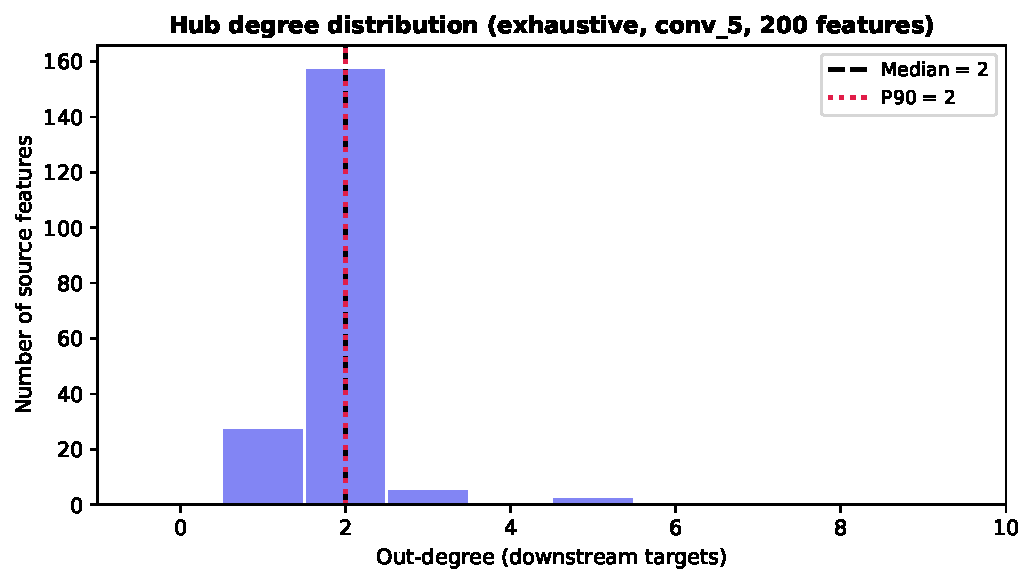
\includegraphics[width=0.6\textwidth]{figures/fig8_hub_degree.pdf}
\caption{\textbf{Heavy-tailed hub distribution from exhaustive tracing.}
Out-degree distribution of 200 source features at conv\_5. Most features
have 1--2 downstream targets; a few hubs have up to 9.}
\label{fig:hub_degree}
\end{figure}

\begin{figure}[ht]
\centering
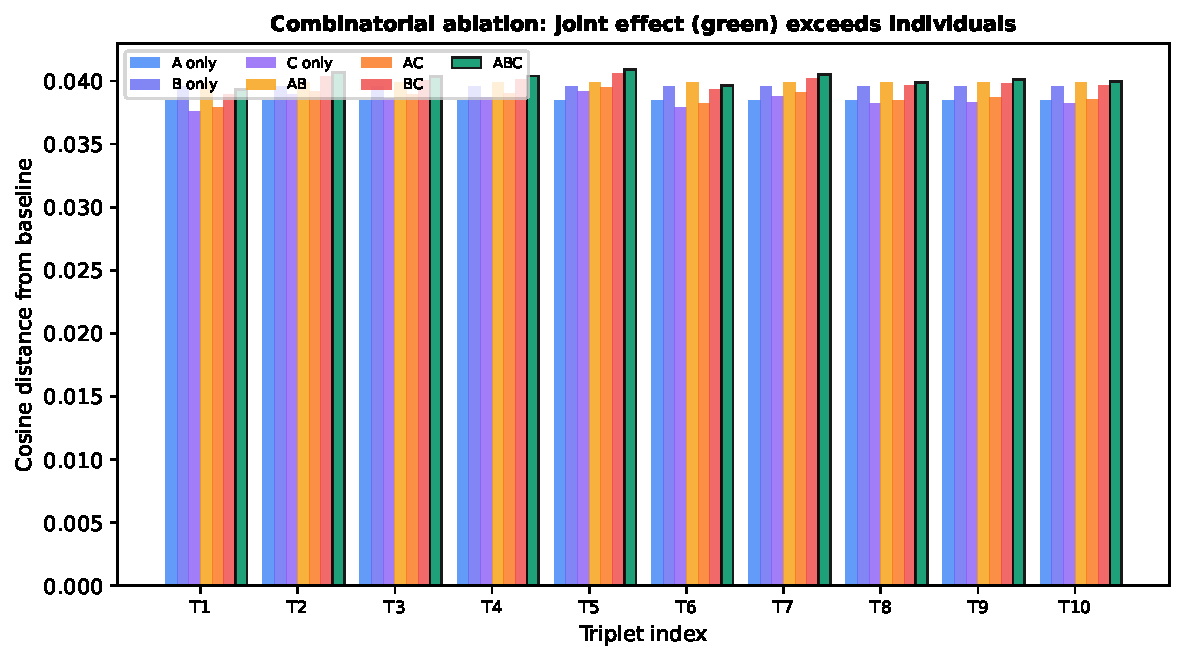
\includegraphics[width=0.75\textwidth]{figures/fig9_combinatorial.pdf}
\caption{\textbf{Combinatorial ablation shows near-additive,
mildly synergistic behavior for one feature pair.} For each triplet,
the joint ABC effect (green) slightly exceeds individual effects,
yielding median $R_{ABC} = 0.958$ (absolute deviation from
independence: 0.042). All 10 triplets share the same
$(\text{feat}_A, \text{feat}_B) = (2107, 2829)$ pair, so this measures
how one SAE pair combines with different third features, not a
general property of SAE triplets. See
Section~\ref{sec:synergy} and Table~\ref{tab:synergy_sensitivity}.}
\label{fig:combinatorial}
\end{figure}

\subsubsection{Feature-triplet ablation: near-additive synergy for one fixed pair}
\label{sec:synergy}

Ablating 10 feature triplets at conv\_0 in all 7 combinations (A, B, C,
AB, AC, BC, ABC) gives median three-way redundancy ratio
$R_{ABC} = 0.958$. A paired bootstrap across the 10 triplets
(10{,}000 resamples) places the median $R_{ABC}$ in a 95\% CI of
$[0.957, 0.966]$.

\textbf{Triplet-selection sensitivity.} Inspection of the 10
triplets reveals that they all share the same
$(\text{feat}_A, \text{feat}_B) = (2107, 2829)$; only the third feature
varies (Table~\ref{tab:synergy_sensitivity}). The ``10-triplet
bootstrap'' is therefore not 10 independent samples of triplet
synergy---it is 10 ways of adding a third feature to one fixed pair.
The narrow CI reflects the stability of this particular pair's
near-additivity, not a general property of triplets in the SAE
dictionary.

\textbf{Magnitude caveat.} The absolute deviation from
independence is only $1 - 0.958 = 0.042$. Component effect sizes are
small ($d_A, d_B, d_C$ median $\approx 0.04$), so the regime is
near-additive and the ratio is sensitive to small numerical
perturbations.

Taken together, these two observations narrow the claim. The present
experiment establishes that \emph{one tested SAE feature pair (F2107,
F2829) participates in near-additive, mildly synergistic triplets
with a diverse set of third features}. A comparison to the
transformer $R = 0.59$ regime as a general GATv2-vs.-transformer
statement would require replicating the experiment on $\geq 3$
independent $(A, B)$ pairs, which we do not do here.

\begin{table}[ht]
\centering
\caption{Triplet-selection structure. All 10 triplets share one
$(A, B)$ pair; only $C$ varies.}
\label{tab:synergy_sensitivity}
\small
\begin{tabular}{lc}
\toprule
Quantity & Value \\
\midrule
Unique $\text{feat}_A$ across triplets & 1 \\
Unique $\text{feat}_B$ across triplets & 1 \\
Unique $\text{feat}_C$ across triplets & 10 \\
Fixed pair $(A, B)$ & (2107, 2829) \\
$R_{AB}$ (std across triplets) & 0 (exact) \\
$R_{ABC}$ range (from choice of $C$) & $0.957$--$0.978$ \\
\bottomrule
\end{tabular}
\end{table}

\subsection{SAE dissociation: shuffled-order control}
\label{sec:dissociation}

To test whether the SAE's biological interpretability depends on the
\emph{learned} aggregator activations rather than on the
gene-expression distribution alone, we train a control SAE on the
same aggregator activations with randomly shuffled cell order
(breaking spatial and biological structure while preserving the
marginal activation distribution). Both SAEs achieve similar
reconstruction quality ($>$99.8\% variance explained).

For this head-to-head comparison we used a 200-feature subset of each
SAE (not the full 2{,}048) and the annotation pipeline was run with a
stricter Enrichr filter than the primary atlas, yielding a real-SAE
annotation rate of \textbf{81\%} (162/200) vs.\ \textbf{40\%} for the
shuffled control ($2.0\times$ ratio). Two points:
\begin{itemize}
\item The 81\% figure is below the 100\% reported for the full 2048-
      feature atlas in Section~\ref{sec:annotation_caveat} because
      this comparison uses a stricter per-feature filter over a
      smaller subset; it is not meant to supersede the 100\% number
      but to compare real vs.\ shuffled at matched settings.
\item Because the per-library FDR$<$0.05 rate against a random
      20-gene panel draw is near 100\% (the panel-saturation ceiling;
      Section~\ref{sec:annotation_caveat}), even the shuffled control
      retains a substantial annotation rate (40\%). The $2\times$
      ratio should therefore be read as a qualitative dissociation,
      not as strong evidence that the SAE captures structure the
      shuffled control cannot reach.
\end{itemize}

\section{Discussion}

\subsection{What Novae has learned: a taxonomy of spatial concepts}
\label{sec:taxonomy}

The SAE atlas suggests that Novae's internal representations
organize into at least four categories of concept, arranged by
their dependence on spatial context:

\textbf{Cell-identity features} (low graph dependency, e.g.\ F208
luminal epithelial, $\text{dep}=0.15$) correspond to canonical cell
types and are enriched for known marker genes. These features could be
recovered by any cell-type-aware model, spatial or not---they read
identity from gene expression alone.

\textbf{Niche features} (moderate graph dependency, e.g.\ F502
vascular niche, $\text{dep}=0.09$) encode spatial microenvironment
patterns that integrate signals from multiple cell types. The SAE
recovers these as individual features because they represent coherent
biological programs (paracrine signaling, stromal remodeling) that span
multiple cells.

\textbf{Context-dependent features} (high graph dependency, e.g.\ F0
T-reg/stromal interface, $\text{dep}_\text{self-loop}=0.47$) are
candidates to encode boundary zones, gradients, and tissue-
architecture patterns that rely on neighborhood information. Of the
1{,}964 features active on the 3-slide feature-permutation corpus,
27\% pass both the self-loop and the feature-permutation threshold
(robust context-dependence), 40\% pass the self-loop test alone
(subject to the architectural-shift confound), 15\% pass the feature-
permutation test alone, and 18\% pass neither
(Section~\ref{sec:graph_ablation}). The 27\% that pass both
tests---equivalently 26\% of the 2{,}024-feature self-loop corpus,
the larger denominator used elsewhere---are our best-supported
candidates for genuinely spatial concepts.

\textbf{Graph-suppressed features} (negative self-loop dependency,
e.g.\ F1885 neutrophils, $\text{dep}_\text{self-loop}=-0.61$)
represent a candidate category: signals that the self-loop ablation
\emph{amplifies} relative to the full graph. A biological reading is
that the graph attention dampens noisy or acute signals
(inflammation, hypoxia) when the neighborhood provides contradictory
evidence. An alternative reading is that the self-loop intervention
shifts the attention softmax normalization in a direction that non-
uniformly raises some features; distinguishing these at the single-
feature level would require running the feature-permutation control
per feature, which is beyond the scope of this work.

\subsection{Implications for foundation-model interpretability}

The pervasive superposition finding (H3: 99.4--100\% of features
misaligned with the top-50 SVD axes) implies that linear
dimensionality reduction alone cannot recover the model's feature
structure. The 64-dimensional aggregator carries features that are
not aligned with its dominant linear directions, so PCA- or SVD-based
interpretation would miss them. This is a narrower statement than
``you cannot interpret Novae by looking at individual neurons''---the
H3 result does not disprove per-neuron monosemanticity directly---
but it does argue that overcomplete dictionaries (such as SAEs) are
a useful complement to direct-neuron analysis when probing a GATv2
aggregator of this dimensionality.

\subsection{Causal circuits propagate through the spatial graph}

The circuit-tracing protocol captures causal effects that propagate
through Novae's graph attention: removing a feature changes the
attention-weighted messages that all affected cells send to their
neighbors, creating a spatially-mediated causal cascade that is
distinct from transformer residual-stream propagation. Within the
single-slide trace, the strength of effects does \emph{not} clearly
attenuate with layer depth; however, the edge counts at gaps $\geq 4$
all originate from conv\_0, and conv\_5---the one mid-depth source
traced---shows mild decay (5, 36, 33 edges for gaps 1--3). We
therefore report the gap-normalized picture
(Table~\ref{tab:gap_normalized},
Section~\ref{sec:attenuation}) and defer any general
attenuation-vs.-no-attenuation statement until tracing from every
source layer.

For the gene-level predictions, the informative statement is that
the 426 predicted pairs co-occur in SAE feature top-gene lists at
$\sim$30$\times$ the random-pair rate
(Section~\ref{sec:gene_pair}): they are not random hits,
but ``novelty vs.\ shared GO term'' is not a calibrated comparison
against that baseline. These predictions remain testable with
spatial perturbation screens at single-cell resolution.

\subsection{The depth story}
\label{sec:depth_story}

Three depth-dependent metrics tell a broadly consistent story.
Compressibility (the SAE's variance-explained) rises from 0.81 at
conv\_0 to 0.998 at the aggregator, with a mid-depth range of
0.81--0.94 at conv\_0--conv\_8 and a dip at conv\_9 (0.903) before the
aggregator jump; the overall trend is upward but not strictly
monotonic. Spatial localization (Moran's $I$) falls from 0.269
(conv\_0) to 0.207 (conv\_8) and 0.119 (aggregator). Cross-layer
feature composition (max $|\cos|$ between successive-layer decoder
columns) rises from 0.019 at conv\_0$\to$conv\_1 to 0.055 at
conv\_8$\to$conv\_9. Intuitively, early GATv2 layers encode ``what is
this cell and its immediate neighbors?'' (high spatial coherence, low
compressibility, low reuse). Later layers ask ``what kind of tissue
environment is this cell in?'' (low spatial coherence, higher
compressibility, more reuse of earlier patterns).

\subsection{Limitations}

\begin{itemize}
\item \textbf{Annotation rate is a ceiling.} Every gene panel cell
      ($G = 487$) against Enrichr libraries hits FDR$<$0.05 at or near
      100\% per library. The ``100\% annotated'' number should always
      be reported together with a random-gene null
      (Section~\ref{sec:annotation_caveat}).
\item \textbf{Cross-tech coherence matches raw-expression baseline.}
      The SAE-feature cross-tech $\rho$ of 0.56 is indistinguishable
      from the raw-expression baseline of 0.57
      (Section~\ref{sec:crosstech}). The feature atlas does
      not demonstrably add tech-invariance beyond the expression data.
\item \textbf{Single-direction ablations need a matched null.} With a
      random-direction null of matched L2 magnitude, 26/50 of the
      tested causally-important features are statistically
      indistinguishable from random directions
      (Section~\ref{sec:proto_ablation}), and 7/50 are below
      the null's lower 95\% CI (i.e., the feature's own direction is
      less effective than a random matched-magnitude perturbation).
      Only 17/50 clear the null's upper CI and should be described as
      direction-specific load-bearing.
\item \textbf{Graph ablation is indirect.} The self-loop protocol
      shifts the aggregation operator as well as removing neighbor
      content. Our feature-permutation control narrows the
      ``context-dependent'' fraction from 67\% to 40\% and identifies
      a 26\% doubly-controlled subset
      (Section~\ref{sec:graph_ablation}). The feature-permutation run
      is on 3 slides (brain, kidney, pancreas; 225{,}867 cells); a
      full replication on the 5-slide self-loop corpus is a future
      extension.
\item \textbf{Circuit tracing is single-slide.} All 439 edges in the
      primary trace come from the brain slide (24k cells). Multi-slide
      replication is outlined in Appendix~\ref{app:scaffolds} but not
      executed here. Cohen's $d > 0.5$ on 24k cells is a small effect
      size, and FDR correction across the tested (source, target)
      pairs is not applied in the primary analysis.
\item \textbf{H5 is not identified.} The three checkpoints have
      non-overlapping gene panels; profile-level correlation cannot
      test convergence. A shared-cell CCA redesign is outlined in
      Appendix~\ref{app:scaffolds}.
\item \textbf{H2 (confound survival) is weak on TopK SAE outputs}
      because most cells have zero activation per feature. The 62\%
      survival rate is an upper bound.
\item \textbf{Perturb-map resolution.} The Visium data is spot-level
      ($\sim$55\,$\mu$m); per-spot composition can drive apparent
      feature-perturbation associations. A composition-regressed
      variant is outlined in Appendix~\ref{app:scaffolds}.
\item \textbf{Cross-technology pairs are disease-vs.-normal in most
      tissues}; the corpus lacks matched conditions across technologies.
\item \textbf{SAE seed stability is not tested in the primary atlas.}
      Feature-specific claims are not verified to be seed-invariant;
      a scaffold for the test is in Appendix~\ref{app:scaffolds}.
\item \textbf{Enrichr annotations are noisy.} Features such as F502
      (``Microfold Cells'' per PanglaoDB but endothelial per domain
      enrichment) and F592 (``Meningeal Cells'' in colon tissue)
      illustrate that the enrichment label can disagree with the
      feature's actual tissue niche. Label-vs-niche discordance is
      systematic and should be reported alongside annotation rate.
\item \textbf{Per-layer enrichment} uses the same top-gene pipeline as
      the aggregator; a decoder-projection approach would be more
      direct for layers where $d = 128$ differs from the gene-embedding
      dimension.
\end{itemize}

\section*{Data and code availability}

\paragraph{Code.}
The complete analysis codebase (TopK SAE module, numbered analysis
scripts, per-control outputs, and paper source) is available at
\url{https://github.com/Biodyn-AI/novae-sae}. The interactive
atlas frontend is at \url{https://github.com/Biodyn-AI/novae-atlas},
deployed at \url{https://biodyn-ai.github.io/novae-atlas/}.

\paragraph{Model checkpoints.}
Novae checkpoints are available from
HuggingFace: \texttt{MICS-Lab/novae-human-0},
\texttt{MICS-Lab/novae-mouse-0}, and \texttt{MICS-Lab/novae-brain-0}
\citep{novae}.

\paragraph{Spatial transcriptomics data.}
The activation corpus uses 15 human tissue slides (4{,}525{,}753 cells)
from the MICS-Lab/novae HuggingFace dataset
(\url{https://huggingface.co/datasets/MICS-Lab/novae}), spanning 13
Xenium \citep{xenium}, 1 MERSCOPE \citep{merfish}, and 1 CosMx slides.
Cross-technology coherence uses 7 additional MERSCOPE slides from the
same dataset. Per-layer analysis uses 3 additional mouse slides (brain,
colon).

\paragraph{Perturbation data.}
The Perturb-map spatial CRISPR screen \citep{perturbmap} (4 mouse lung
Visium sections) was obtained from GEO accession GSE193460.

\paragraph{Enrichment databases.}
Gene set enrichment uses locally cached libraries from Enrichr
\citep{enrichr}: GO Biological Process 2023 \citep{go2021}, KEGG 2021
\citep{kegg2000}, Reactome 2022 \citep{reactome2020}, PanglaoDB
Augmented 2021 \citep{panglao}, and CellMarker Augmented 2021
\citep{cellmarker2019}.

\appendix
\section{Planned extensions}
\label{app:scaffolds}

The following experiments are outlined as runnable scripts in the
code repository. Each requires forward-pass compute or model
retraining that is beyond the scope of this paper; we list them to
document the complete analysis plan.

\paragraph{Multi-slide circuit replication.}
Re-running the circuit-tracing protocol on pancreas and kidney slides
with the same source/target layers as the primary brain trace, to
report edge Jaccard reproducibility across tissues and an FDR-
corrected edge set.

\paragraph{SAE seed stability.}
Retraining the aggregator SAE with additional random seeds on a
500k-cell subsample, with Hungarian-matched decoder-column overlap
against the primary atlas and per-feature best-match scores for the
50 causally-tested features.

\paragraph{Random-initialized Novae baseline.}
Extracting aggregator activations from a randomly-initialized Novae
checkpoint of the same architecture, training an SAE on those
activations, and comparing annotation rate and context dependency to
the trained-model SAE, to separate architecture-only inductive bias
from learned structure.

\paragraph{Perturb-map composition control.}
Regressing out per-spot cell-type composition before testing SAE
feature--perturbation associations, to control for the confound that
Visium spots of $\sim$55\,$\mu$m span multiple cells.

\paragraph{Shared-cell CCA for cross-checkpoint comparison.}
Forward-passing a shared set of cells on an intersection gene panel
through all three checkpoints and aligning latent spaces via CCA,
replacing the profile-level correlation (which is not identified by
the different gene panels) with a properly designed convergence test.

\section*{Acknowledgments}

This work was enabled by the MICS-Lab/novae dataset and the Novae model
checkpoints released by Blampey et al.\ under open licenses.

\bibliographystyle{apalike}
\begin{thebibliography}{99}

\bibitem[Anselin, 1995]{anselin1995}
Anselin, L.\ (1995).
\newblock Local indicators of spatial association---LISA.
\newblock {\em Geographical Analysis}, 27(2):93--115.

% --- Contrastive / self-supervised learning ---

\bibitem[Bills et~al., 2023]{bills2023}
Bills, S., Cammarata, N., Mossing, D., et~al.\ (2023).
\newblock Language models can explain neurons in language models.
\newblock {\em OpenAI Blog}.

\bibitem[Blampey et~al., 2025]{novae}
Blampey, Q., Benkirane, H., Bercovici, N., et~al.\ (2025).
\newblock Novae: a graph foundation model for spatial omics.
\newblock {\em Nature Methods}, s41592-025-02899-6.

\bibitem[Blondel et~al., 2008]{louvain2008}
Blondel, V.D., Guillaume, J.-L., Lambiotte, R., Lefebvre, E.\ (2008).
\newblock Fast unfolding of communities in large networks.
\newblock {\em Journal of Statistical Mechanics}, 2008(10):P10008.

\bibitem[Bricken et~al., 2023]{bricken2023}
Bricken, T., Templeton, A., Batson, J., et~al.\ (2023).
\newblock Towards monosemanticity: Decomposing language models with
  dictionary learning.
\newblock {\em Anthropic Research}.

\bibitem[Brody et~al., 2022]{gatv2}
Brody, S., Alon, U., Yahav, E.\ (2022).
\newblock How attentive are graph attention networks?
\newblock {\em ICLR 2022}.

\bibitem[Caron et~al., 2020]{swav}
Caron, M., Misra, I., Mairal, J., Goyal, P., Bojanowski, P., Joulin, A.\ (2020).
\newblock Unsupervised learning of visual features by contrasting cluster
  assignments.
\newblock {\em NeurIPS 2020}.

\bibitem[Chen et~al., 2015]{merfish}
Chen, K.H., Boettiger, A.N., Moffitt, J.R., Wang, S., Zhuang, X.\ (2015).
\newblock Spatially resolved, highly multiplexed RNA profiling in single
  cells.
\newblock {\em Science}, 348(6233):aaa6090.

\bibitem[Chen et~al., 2020]{simclr2020}
Chen, T., Kornblith, S., Norouzi, M., Hinton, G.E.\ (2020).
\newblock A simple framework for contrastive learning of visual representations.
\newblock {\em ICML 2020}, pages 1597--1607.

\bibitem[Conmy et~al., 2023]{conmy2023}
Conmy, A., Mavor-Parker, A.N., Lynch, A., Heimersheim, S., Garriga-Alonso, A.\ (2023).
\newblock Towards automated circuit discovery for mechanistic interpretability.
\newblock {\em NeurIPS 2023}.

\bibitem[Cui et~al., 2024]{scgpt}
Cui, H., Wang, C., Maan, H., et~al.\ (2024).
\newblock scGPT: toward building a foundation model for single-cell
  multi-omics using generative AI.
\newblock {\em Nature Methods}, 21(8):1470--1480.

\bibitem[Cunningham et~al., 2024]{cunningham2023}
Cunningham, H., Ewart, A., Riggs, L., Huben, R., Sharkey, L.\ (2024).
\newblock Sparse autoencoders find highly interpretable features in
  language models.
\newblock {\em arXiv:2309.08600}.

\bibitem[Dhainaut et~al., 2022]{perturbmap}
Dhainaut, M., Rose, S.A., Bhatt, D., et~al.\ (2022).
\newblock Spatial CRISPR genomics identifies regulators of the tumor
  microenvironment.
\newblock {\em Cell}, 185(5):757--774.

\bibitem[Elhage et~al., 2022]{elhage2022superposition}
Elhage, N., Hume, T., Olsson, C., et~al.\ (2022).
\newblock Toy models of superposition.
\newblock {\em arXiv:2209.10652}.

\bibitem[Elhage et~al., 2021]{elhage2021}
Elhage, N., Nanda, N., Olsson, C., et~al.\ (2021).
\newblock A mathematical framework for transformer circuits.
\newblock {\em Transformer Circuits Thread}.

\bibitem[Fey and Lenssen, 2019]{pyg}
Fey, M., Lenssen, J.E.\ (2019).
\newblock Fast graph representation learning with PyTorch Geometric.
\newblock {\em ICLR Workshop on Representation Learning on Graphs
  and Manifolds}.

\bibitem[Franz\'en et~al., 2019]{panglao}
Franz\'en, O., Gan, L.-M., Bj\"orkegren, J.L.M.\ (2019).
\newblock PanglaoDB: a web server for exploration of mouse and human
  single-cell RNA sequencing data.
\newblock {\em Database}, 2019:baz046.

\bibitem[Gao et~al., 2024]{gao2024}
Gao, L., la~Tour, T.D., Tillman, H., Goh, G., Troll, R., et~al.\ (2024).
\newblock Scaling and evaluating sparse autoencoders.
\newblock {\em arXiv:2406.04093}.

\bibitem[{Gene Ontology Consortium}, 2021]{go2021}
{Gene Ontology Consortium} (2021).
\newblock The Gene Ontology resource: enriching a GOld mine.
\newblock {\em Nucleic Acids Research}, 49(D1):D325--D334.

\bibitem[Getis and Ord, 1992]{getis1992}
Getis, A., Ord, J.K.\ (1992).
\newblock The analysis of spatial association by use of distance statistics.
\newblock {\em Geographical Analysis}, 24(3):189--206.

\bibitem[Hao et~al., 2024]{hao2024}
Hao, M., Gong, J., Zeng, X., et~al.\ (2024).
\newblock Large-scale foundation model on single-cell transcriptomics.
\newblock {\em Nature Methods}, 21:1481--1491.

\bibitem[He et~al., 2020]{moco2020}
He, K., Fan, H., Wu, Y., Xie, S., Girshick, R.\ (2020).
\newblock Momentum contrast for unsupervised visual representation learning.
\newblock {\em CVPR 2020}.

% --- Analysis tools ---

\bibitem[Janesick et~al., 2023]{xenium}
Janesick, A., Shelansky, R., Engblom, C., et~al.\ (2023).
\newblock High resolution mapping of the breast cancer tumor microenvironment
  using integrated single cell, spatial and in situ analysis of FFPE tissue.
\newblock {\em Nature Communications}, 14:8318.

\bibitem[Jassal et~al., 2020]{reactome2020}
Jassal, B., Matthews, L., Viteri, G., et~al.\ (2020).
\newblock The Reactome pathway knowledgebase.
\newblock {\em Nucleic Acids Research}, 48(D1):D498--D503.

\bibitem[Kanehisa and Goto, 2000]{kegg2000}
Kanehisa, M., Goto, S.\ (2000).
\newblock KEGG: Kyoto Encyclopedia of Genes and Genomes.
\newblock {\em Nucleic Acids Research}, 28(1):27--30.

\bibitem[Kendiukhov, 2026]{sae_atlas}
Kendiukhov, I.\ (2026).
\newblock Sparse autoencoder atlases for single-cell foundation models.
\newblock {\em arXiv:2603.02952}.

\bibitem[Kipf and Welling, 2017]{kipf2017}
Kipf, T.N., Welling, M.\ (2017).
\newblock Semi-supervised classification with graph convolutional networks.
\newblock {\em ICLR 2017}.

\bibitem[Kuleshov et~al., 2016]{enrichr}
Kuleshov, M.V., Jones, M.R., Rouillard, A.D., et~al.\ (2016).
\newblock Enrichr: a comprehensive gene set enrichment analysis web server
  2016 update.
\newblock {\em Nucleic Acids Research}, 44(W1):W90--W97.

\bibitem[Li et~al., 2022]{li2022gnn}
Li, M.M., Huang, K., Zitnik, M.\ (2022).
\newblock Graph representation learning in biomedicine and healthcare.
\newblock {\em Nature Biomedical Engineering}, 6:1353--1369.

\bibitem[Longo et~al., 2021]{longo2021}
Longo, S.K., Guo, M.G., Ji, A.L., Khavari, P.A.\ (2021).
\newblock Integrating single-cell and spatial transcriptomics to elucidate
  intercellular tissue dynamics.
\newblock {\em Nature Reviews Genetics}, 22:627--644.

\bibitem[Makhzani and Frey, 2014]{makhzani2014}
Makhzani, A., Frey, B.J.\ (2014).
\newblock $k$-Sparse Autoencoders.
\newblock {\em ICLR 2014}.

% --- Mechanistic interpretability ---

\bibitem[Marks et~al., 2025]{marks2025}
Marks, S., Rager, C., Michaud, E.J., Belinkov, Y., Bau, D., Mueller, A.\ (2025).
\newblock Sparse feature circuits: discovering and editing interpretable
  causal graphs in language models.
\newblock {\em ICLR 2025}.

\bibitem[Marx, 2021]{marx2021}
Marx, V.\ (2021).
\newblock Method of the Year: spatially resolved transcriptomics.
\newblock {\em Nature Methods}, 18:9--14.

\bibitem[McInnes et~al., 2018]{umap2018}
McInnes, L., Healy, J., Melville, J.\ (2018).
\newblock UMAP: Uniform manifold approximation and projection for dimension
  reduction.
\newblock {\em arXiv:1802.03426}.

% --- Foundational ---

\bibitem[Moran, 1950]{moran1950}
Moran, P.A.P.\ (1950).
\newblock Notes on continuous stochastic phenomena.
\newblock {\em Biometrika}, 37(1/2):17--23.

\bibitem[Moses and Pachter, 2022]{moses2022}
Moses, L., Pachter, L.\ (2022).
\newblock Museum of spatial transcriptomics.
\newblock {\em Nature Methods}, 19:534--546.

\bibitem[Olah et~al., 2020]{olah2020}
Olah, C., Cammarata, N., Schubert, L., Goh, G., Petrov, M., Carter, S.\ (2020).
\newblock Zoom In: An introduction to circuits.
\newblock {\em Distill}, 5(3):e00024.001.

% --- Spatial transcriptomics ---

\bibitem[Rao et~al., 2021]{rao2021}
Rao, A., Barkley, D., Fran\c{c}a, G.S., Yanai, I.\ (2021).
\newblock Exploring tissue architecture using spatial transcriptomics.
\newblock {\em Nature}, 596:211--220.

% --- Single-cell foundation models ---

\bibitem[Rosen et~al., 2023]{rosen2023}
Rosen, Y., Roohani, Y., Agarwal, A., et~al.\ (2023).
\newblock Universal cell embeddings: a foundation model for cell biology.
\newblock {\em bioRxiv}, 2023.11.28.568918.

% --- Graph neural networks ---

\bibitem[Sharkey et~al., 2022]{sharkey2022}
Sharkey, L., Braun, D., Millidge, B.\ (2022).
\newblock Taking features out of superposition with sparse autoencoders.
\newblock {\em Alignment Forum}.

\bibitem[Subramanian et~al., 2005]{gsea2005}
Subramanian, A., Tamayo, P., Mootha, V.K., et~al.\ (2005).
\newblock Gene set enrichment analysis: a knowledge-based approach for
  interpreting genome-wide expression profiles.
\newblock {\em PNAS}, 102(43):15545--15550.

\bibitem[Templeton et~al., 2024]{templeton2024}
Templeton, A., Conerly, T., Marcus, J., et~al.\ (2024).
\newblock Scaling monosemanticity: Extracting interpretable features
  from Claude 3 Sonnet.
\newblock {\em Anthropic Research}.

\bibitem[Theodoris et~al., 2023]{geneformer}
Theodoris, C.V., Xiao, L., Chopra, A., et~al.\ (2023).
\newblock Transfer learning enables predictions in network biology.
\newblock {\em Nature}, 618(7965):616--624.

\bibitem[Traag et~al., 2019]{leiden}
Traag, V.A., Waltman, L., van~Eck, N.J.\ (2019).
\newblock From Louvain to Leiden: guaranteeing well-connected communities.
\newblock {\em Scientific Reports}, 9:5233.

\bibitem[Vaswani et~al., 2017]{vaswani2017}
Vaswani, A., Shazeer, N., Parmar, N., et~al.\ (2017).
\newblock Attention is all you need.
\newblock {\em NeurIPS 2017}.

\bibitem[Veli\v{c}kovi\'{c} et~al., 2018]{velickovic2018}
Veli\v{c}kovi\'{c}, P., Cucurull, G., Casanova, A., Romero, A.,
Li\`{o}, P., Bengio, Y.\ (2018).
\newblock Graph attention networks.
\newblock {\em ICLR 2018}.

% --- Biological databases ---

\bibitem[Williams et~al., 2022]{williams2022}
Williams, C.G., Lee, H.J., Asatsuma, T., Vento-Tormo, R., Haque, A.\ (2022).
\newblock An introduction to spatial transcriptomics for biomedical research.
\newblock {\em Genome Medicine}, 14:68.

\bibitem[Wolf et~al., 2018]{scanpy}
Wolf, F.A., Angerer, P., Theis, F.J.\ (2018).
\newblock SCANPY: large-scale single-cell gene expression data analysis.
\newblock {\em Genome Biology}, 19:15.

\bibitem[Yang et~al., 2022]{yang2022}
Yang, F., Wang, W., Wang, F., et~al.\ (2022).
\newblock scBERT as a large-scale pretrained deep language model for cell
  type annotation of single-cell RNA-seq data.
\newblock {\em Nature Machine Intelligence}, 4:852--866.

\bibitem[Zhang et~al., 2019]{cellmarker2019}
Zhang, X., Lan, Y., Xu, J., et~al.\ (2019).
\newblock CellMarker: a manually curated resource of cell markers in
  human and mouse.
\newblock {\em Nucleic Acids Research}, 47(D1):D721--D728.

% --- Spatial statistics ---

\end{thebibliography}

\end{document}
